\section{Scaffolding Improvement}
\label{sec:Scaffolding_Improvement}

This section analyzes the scaffolding improvement paradigm for FM-based agents, where we approach this by decomposing the agent's operational scaffold into core components. This workflow begins with receiving and interpreting instructions, then contextualizes them using internal knowledge and memory, proceeds to executing actions in the world, and ultimately evolves the overall operational structure. 

Formally, as established in Section ~\ref{sec:Definitions}, scaffolding improvement corresponds to transitions that modify the operational scaffold while explicitly keeping the foundation-model parameters frozen ($\theta_{t+1}=\theta_{t}$). Driven by an execution-derived learning signal $\mathcal{S}_{t}$ (e.g., task outcomes, critique, or execution errors), the update is formalized as $\Sigma_{t+1}=\IMPROVE_{\Sigma}(\Sigma_{1:t};\mathcal{S}_{t})$. By maintaining a version history ($\Sigma_{1:t}$), the system inherently supports validation and rollback against harmful modifications across all components. We structure the discussion by increasing depth of architectural intervention. Concretely, we instantiate the scaffolding as $\Sigma_{t}:=(p_{t},m_{t},\mathcal{T}_{t},g_{t})$, where $p_{t}$ denotes the prompt template, $m_{t}$ the internal memory, $\mathcal{T}_{t}$ the external tool set, and $g_{t}$ the control logic. Algorithm~\ref{alg:scaffolding_improvement} summarizes the generic improvement loop across these components:


\begin{itemize}[leftmargin=*]
    \item \textbf{Prompt-based improvement} (Section~\ref{sec:Prompt_Optimization}) targets the agent's input and instruction layer, formalized as $p_{t+1}=\IMPROVE_{p}(p_{1:t};\mathcal{S}_t)$.  As the primary semantic interface through which the agent perceives its tasks, optimizing the prompt provides a direct way to refine task communication, objectives, and constraints without altering the internal parameters of the foundation model.

    
    \item \textbf{Memory-based improvement} (Section~\ref{sec:Memory}) equips the agent with an evolving internal cognitive resource, updated via $m_{t+1}=\IMPROVE_{m}(m_{1:t};\mathcal{S}_t)$. 
    By dynamically storing, pruning, and retrieving past experiences, the agent shifts from memoryless execution to cumulative learning, supporting long-horizon reasoning and trustworthy adaptation.  

    
    \item \textbf{Tool-based improvement} (Section~\ref{sec:Tool}) strengthens the agent's execution interface through the update $\mathcal{T}_{t+1}=\IMPROVE_{\mathcal{T}}(\mathcal{T}_{1:t};\mathcal{S}_t)$. 
    By autonomously refining and managing external callable modules (e.g., web search, code interpreters), the agent translates internal decisions into precise, executable actions, effectively extending its capabilities beyond the native limits of the foundation model.

    
    \item \textbf{Full scaffolding improvement} (Section~\ref{sec:Full_Scaffolding}) represents the most profound level of architectural intervention, formalized as $\Sigma_{t+1}=\IMPROVE_{\Sigma}(\Sigma_{1:t};\mathcal{S}_t)$. 
    By treating the entire codebase and operational logic as a mutable substrate, the agent dynamically reconfigures how its perception, reasoning, and execution faculties are integrated into a coherent whole.
\end{itemize}

\textbf{Crucially, these intervention types are compositional rather than mutually exclusive:} a single update can edit multiple scaffold components simultaneously, and full-scaffolding methods naturally subsume component-level edits while adding archive-based exploration and stronger acceptance tests.

% ==============algorithm pseudo-code================
\AlgoSel=4 % Algorithm 1 v3 (aligned + more inclusive, no overflow)
\ifnum\AlgoSel=3
\begin{wrapfigure}{r}{0.52\columnwidth}
\vspace{-\intextsep}
\centering

\scalebox{0.52}{%
\begin{minipage}{\columnwidth}
\begin{mdframed}[
  backgroundcolor=algobg,
  roundcorner=5pt,
  linewidth=0pt,
  innerleftmargin=4pt,
  innerrightmargin=4pt,
  innertopmargin=4pt,
  innerbottommargin=4pt
]
\begingroup
\SetAlFnt{\large}   
\SetAlCapFnt{\large}  
\SetAlCapNameFnt{\large} 
\begin{algorithm}[H]
\caption{Foundation\mbox{-}Model Improvement}
\label{alg:foundation_model_improvement}

\SetKwInOut{Input}{Input}
\SetKwInOut{Output}{Output}
\Input{Initial agent state $\mathcal{A}_0=(\theta_0,\Sigma)$; maximum iterations $T$}
\Output{Improved agent $\mathcal{A}_T=(\theta_T,\Sigma)$}

\BlankLine
\For{$t \leftarrow 0$ \KwTo $T-1$}{

  \textcolor{RoyalBlue}{\tcp{1) Construct or collect learning signal $\mathcal{S}_t$}}
  $\mathcal{S}_t \leftarrow \emptyset$

  \If{subcategory includes intrinsic generative demonstrations}{%
    $\mathcal{S}_t \leftarrow \mathcal{S}_t \cup \textsc{GenerateDemonstrations}(\mathcal{A}_t)$
    \tcp*{\S \ref{sec:Intrinsic_Generative_Demonstrations}}
  }
  \If{subcategory includes intrinsic evaluative feedback}{%
    $\mathcal{S}_t \leftarrow \mathcal{S}_t \cup \textsc{GenerateEvaluativeFeedback}(\mathcal{A}_t)$
    \tcp*{\S \ref{sec:Intrinsic_Evaluative_Feedback}}
  }
  \If{subcategory includes extrinsic exploratory experience}{%
    $\mathcal{S}_t \leftarrow \mathcal{S}_t \cup \textsc{CollectExperience}(\mathcal{A}_t,\text{env})$
    \tcp*{\S \ref{sec:Extrinsic_Exploratory_Experience}}
  }

  \textcolor{gray}{\tcp{Optional: quality control / weighting of signals}}
  $\mathcal{S}_t \leftarrow \textsc{FilterOrWeight}(\mathcal{S}_t)$

  \textcolor{RoyalBlue}{\tcp{2) Parameter update}}
  $\theta_{t+1} \leftarrow \textsc{Update}(\theta_{1:t},\mathcal{S}_t)$

  \textcolor{RoyalBlue}{\tcp{3) State update}}
  $\mathcal{A}_{t+1} \leftarrow (\theta_{t+1},\Sigma)$

  \If{\textsc{Converged}($\mathcal{A}_{t+1}$)}{break}
}
\Return{$\mathcal{A}_T$}
\end{algorithm}
\endgroup
\end{mdframed}
\end{minipage}%
}

\vspace{-10pt}
\end{wrapfigure}
\fi


% Algorithm 2 v3 (aligned + more inclusive, no overflow)
\ifnum\AlgoSel=4
\begin{wrapfigure}{r}{0.52\columnwidth}
\vspace{-\intextsep}
\centering

\scalebox{0.52}{%
\begin{minipage}{\columnwidth}
\begin{mdframed}[
  backgroundcolor=algobg,
  roundcorner=5pt,
  linewidth=0pt,
  innerleftmargin=4pt,
  innerrightmargin=4pt,
  innertopmargin=4pt,
  innerbottommargin=4pt
]
\begingroup
\SetAlFnt{\large}   
\SetAlCapFnt{\large}  
\SetAlCapNameFnt{\large} 
\begin{algorithm}[H]
\caption{Scaffolding Improvement}
\label{alg:scaffolding_improvement}

\SetKwInOut{Input}{Input}
\SetKwInOut{Output}{Output}
\Input{Initial agent state $\mathcal{A}_0=(\theta,\Sigma_0)$; max iterations $T$}
\Output{Improved agent $\mathcal{A}_T=(\theta,\Sigma_T)$}

\BlankLine
\For{$t \leftarrow 0$ \KwTo $T-1$}{

  \textcolor{RoyalBlue}{\tcp{1) Collect scaffolding learning signal $\mathcal{S}_t$}}
  $\mathcal{S}_t \leftarrow \textsc{InteractAndEvaluate}(\mathcal{A}_t,\text{env})$
  \tcp*{\footnotesize traces, critiques, success/failure, cost}

  \textcolor{gray}{\tcp{Optional: quality control / weighting of signals}}
  $\mathcal{S}_t \leftarrow \textsc{FilterOrWeight}(\mathcal{S}_t)$

  \textcolor{RoyalBlue}{\tcp{2) Scaffolding update (keep $\theta$ fixed)}}
  \uIf{subcategory = Full scaffolding}{%
    $\Sigma_{t+1} \leftarrow \IMPROVE_{\Sigma}(\Sigma_{1:t};\mathcal{S}_t)$
    \tcp*{\S~\ref{sec:Full_Scaffolding}}
  }
  \Else{%
    $p_{t+1} \leftarrow p_t$; $m_{t+1} \leftarrow m_t$; $\mathcal{T}_{t+1} \leftarrow \mathcal{T}_t$

    \If{subcategory includes Prompt-based}{%
      $p_{t+1} \leftarrow \IMPROVE_{p}(p_t;\mathcal{S}_t)$
      \tcp*{\S~\ref{sec:Prompt_Optimization}}
    }
    \If{subcategory includes Memory-based}{%
      $m_{t+1} \leftarrow \IMPROVE_{m}(m_t;\mathcal{S}_t)$
      \tcp*{\S~\ref{sec:Memory}}
    }
    \If{subcategory includes Tool-based}{%
      $\mathcal{T}_{t+1} \leftarrow \IMPROVE_{\mathcal{T}}(\mathcal{T}_t;\mathcal{S}_t)$
      \tcp*{\S~\ref{sec:Tool}}
    }

    $\Sigma_{t+1} \leftarrow (p_{t+1},\, m_{t+1},\, \mathcal{T}_{t+1})$
  }

  \textcolor{RoyalBlue}{\tcp{3) State update}}
  $\mathcal{A}_{t+1} \leftarrow (\theta,\Sigma_{t+1})$
}
\Return{$\mathcal{A}_T$}
\end{algorithm}
\endgroup
\end{mdframed}
\end{minipage}%
}

\vspace{-16pt}
\end{wrapfigure}
\fi
% ==============algorithm pseudo-code================


\subsection{Prompt}
\label{sec:Prompt_Optimization}
The prompt serves as the agent's core behavioral prior, defining how the foundation model parses its environment. Prompt optimization is therefore a central and highly accessible form of scaffolding improvement. While early methods relied on manual heuristic tuning, the field is rapidly developed toward automated, signal-driven improvement loops. Central to this development is the transition from scalar-based feedback to rich, structured linguistic critiques. By leveraging natural-language gradients, these systems now facilitate targeted, iterative updates that mirror the precision of gradient-based optimization in higher-dimensional strategy spaces.

In this section, prompt primarily refers to structural instruction layers that are reused across interactions, such as system prompts or stable policy templates. A closely related line of work optimizes context construction, including exemplar selection, retrieval assembly, and the maintenance of long-term playbooks. Although both are scaffold-level updates, they differ in target: optimizing a system prompt alters the agent’s core behavioral prior, whereas context optimization refines the dynamic conditioning of specific interactions. When discussing representative systems, we will explicitly indicate which object is updated.

As shown in Fig.~\ref{fig:prompt}, we categorize prompt refinement methods based on the form and richness of the learning signal $\mathcal{S}_t$. This yields four paradigms: (1) \textit{Scalar-Feedback Optimization}, where $\mathcal{S}_t$ is a scalar performance score such as accuracy or reward;
(2) \textit{Qualitative-Feedback Refinement}, where $\mathcal{S}_t$ is a natural-language critique or suggestion for providing interpretable revision guidance;
(3) \textit{Population-Based Evolution}, where $\mathcal{S}_t$ consists of population-level fitness evaluation and selection signals over a set of candidate prompts;
and (4) \textit{Textual Gradient Optimization}, where $\mathcal{S}_t$ is structured directional guidance, often expressed as a textual gradient that specifies how the prompt should be revised. As listed in Table~\ref{tab:prompt_optimization_paradigms}, we further summarize representative systems and trade-offs across paradigms.


\begin{figure*}[ht]
    \centering
    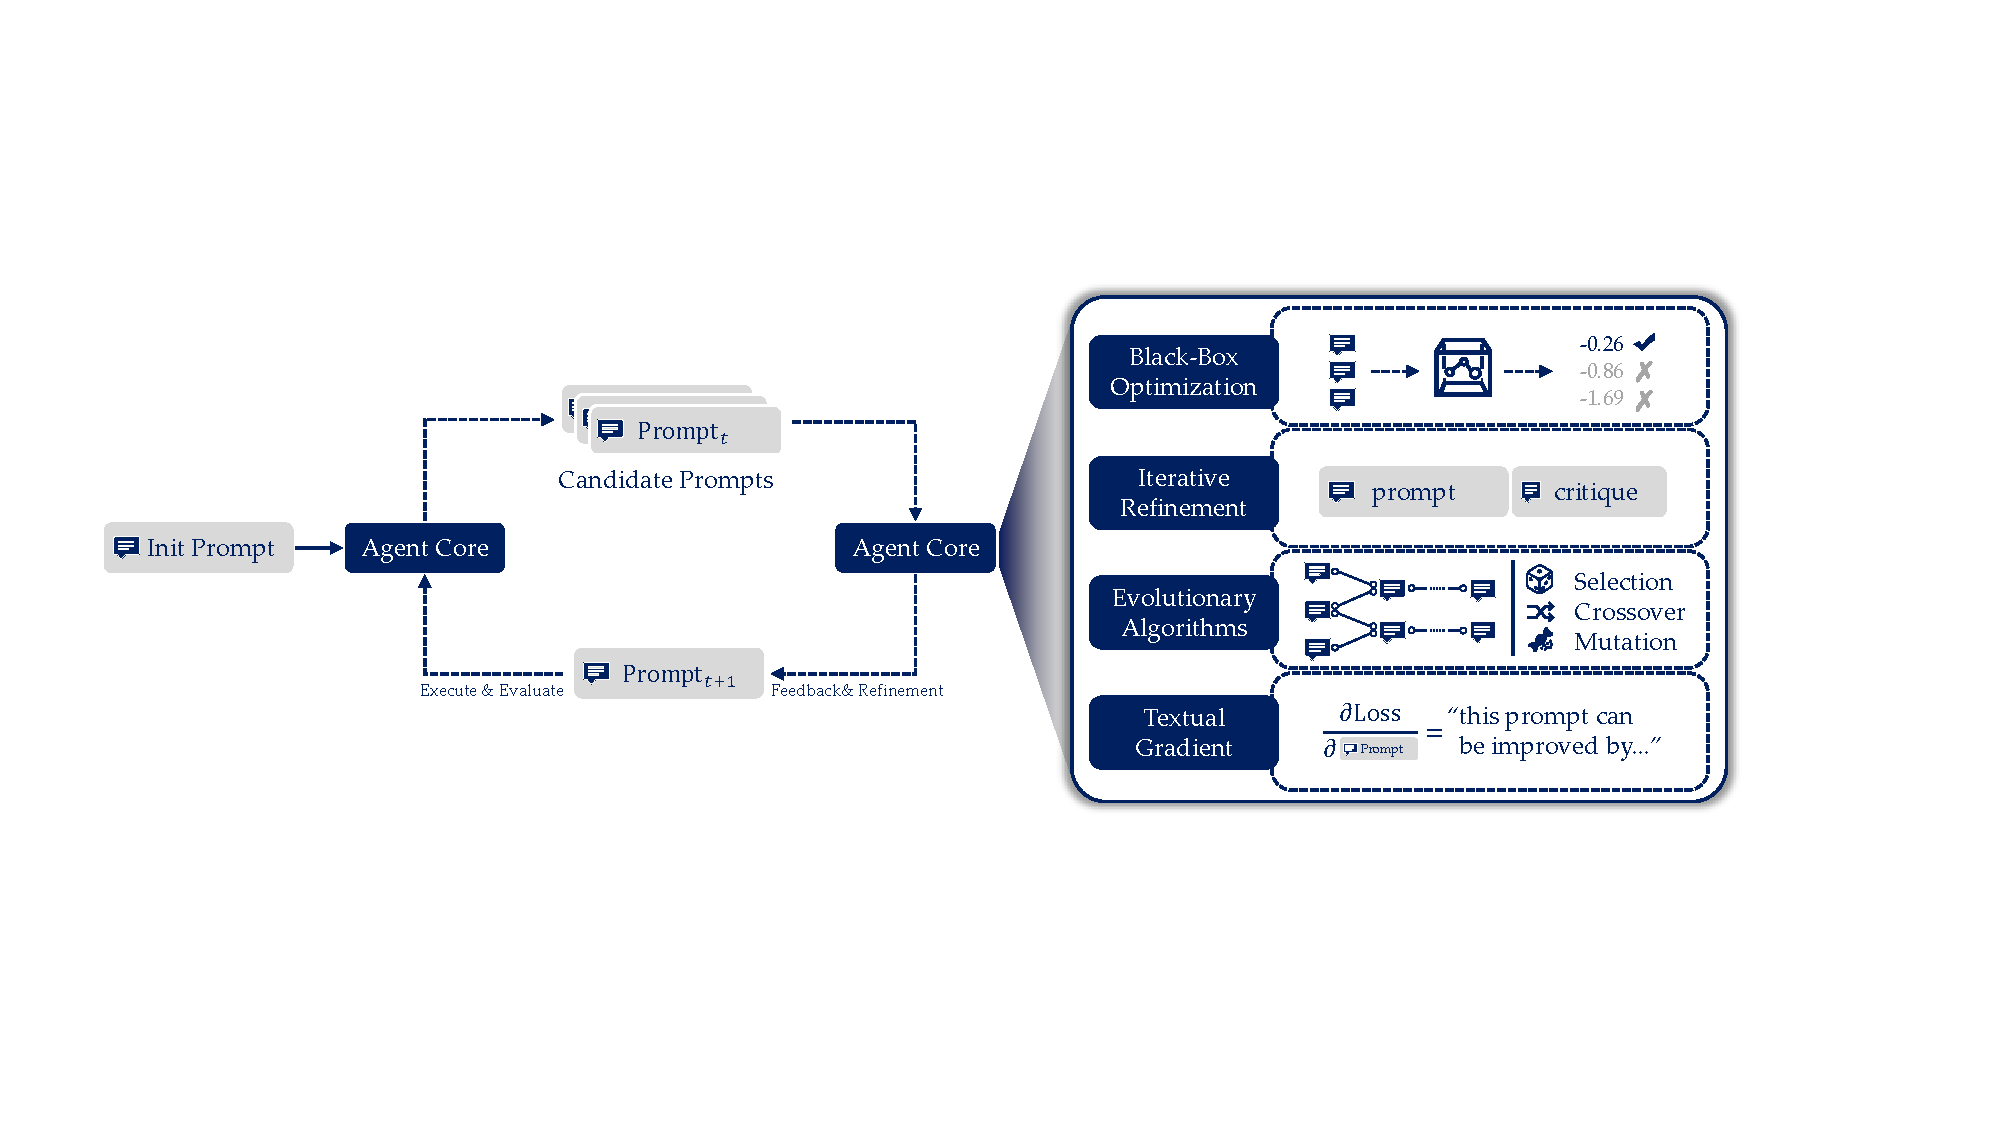
\includegraphics[width=1\linewidth]{fig/fig-prompt.pdf}
    \caption{Prompt refinement as a self-improvement loop and its four paradigms, organized by the learning signal $\mathcal{S}_t$.}
    \label{fig:prompt}
\end{figure*}



\subsubsection{Scalar-Feedback Optimization}
\label{sec:Scalar_Feedback_Optimization}

Early approaches to prompt optimization usually rely on task-level quantitative metrics to evaluate candidates \citep{zhou2022large}. The core objective can be formally defined as finding an optimal prompt $p^*$ from a discrete space of possible prompts $\mathcal{P}$ that maximizes a scalar performance score (e.g., task accuracy or reward):
\begin{equation}p^* = \arg\max_{p \in \mathcal{P}} f(p),
\end{equation}
where $f(p)$ represents the evaluation function. In the context of our scaffolding improvement framework, this scalar score is used to constitutes the learning signal ($\mathcal{S}_t = f(p_t)$). Considering $\mathcal{S}_t$ is non-directional, providing only a magnitude of success without explanatory context, these methods typically rely on structured search algorithms to navigate the discrete text space. APE pioneered this paradigm by using an LLM to propose instruction candidates, subsequently selecting the best one based on empirical evaluation scores via simple search \citep{zhou2022large}. Building on this, OPRO formalized a more contextualized search by constructing a meta-prompt that includes a trajectory of previously evaluated prompts alongside their scalar scores, indirectly guiding the LLM to propose higher-scoring candidates in subsequent iterations \citep{yang2023large}.


Besides, researchers have adapted advanced derivative-free optimization algorithms to operate strictly on scalar feedback. For instance, RL-based frameworks like RLPrompt treat prompt generation as a discrete reinforcement learning problem, directly optimizing a reward signal derived from downstream task accuracy \citep{deng2022rlprompt}. Similarly, to improve the sample efficiency of exploring the discrete text space, methods like InstructZero map prompts into a continuous latent space, leveraging Bayesian Optimization to predict and maximize scalar task rewards efficiently \citep{cheninstructzero}. Recent systems like BPO (Black-Box Prompt Optimization) further extend this score-driven paradigm to human preference alignment, using scalar preference scores to optimize user inputs without altering the underlying model weights \citep{cheng2024black}.


\subsubsection{Qualitative-Feedback Refinement}
\label{sec:Qualitative_Feedback_Refinement}

Building upon scalar-driven methods, a more nuanced approach focuses on iterative refinement using qualitative, interpretable feedback. Instead of a single score, the learning signal ($\mathcal{S}_t$) manifests as a textual critique, error analysis, or natural-language suggestion, denoted as $c_t$. This richer signal allows for a targeted revision process, formally modeled as an iterative loop where each new prompt $p_{t+1}$ is a function of the previous prompt $p_t$ and its corresponding qualitative feedback $c_t$:
\begin{equation}p_{t+1} = \text{Refine}(p_t, c_t),
\end{equation}
where $c_t$ is typically generated by an evaluator or the LLM itself based on historical execution: $c_t = \text{Critique}(\text{Output}(p_t))$. While foundational paradigms like Self-Refine \citep{madaan2023self} and multi-agent debate \citep{liang2023debate} demonstrated the power of self-critique for transient output correction, recent scaffolding improvements persist this qualitative feedback to update the agent's prompting policy or instructional context. One prominent direction leverages error-driven qualitative analysis. Reflexion, for example, enables an agent to generate ``verbal introspection'' upon task failure, storing these qualitative reflections in memory to explicitly guide and constrain subsequent prompting attempts \citep{shinn2023reflexionlanguageagentsverbal}. Expanding on this diagnostic capability, MAPS introduces an automated, LLM-tailored prompt optimization framework that explicitly induces and validates reusable natural-language rules from failure cases. By iteratively injecting these qualitative insights into the prompt, MAPS substantially optimizes the policy for complex tasks like unit test generation \citep{gao2025promptalchemistautomatedllmtailored}. Similarly, inspired by Chain of Hindsight (CoH), agents can learn from textual contrasts by reviewing a history of past attempts accompanied by qualitative evaluations \citep{liu2023chain}. Another critical direction involves evolving the instructional context. To manage the growing complexity of text-based critiques, ACE introduces an agentic context engineering framework with a modular \textit{Generator–Reflector–Curator} pipeline. ACE treats prompts and memory as evolving text playbooks, actively curating qualitative feedback while mitigating brevity bias and context collapse \citep{zhang2025agenticcontextengineeringevolving}. In specific domain applications, systems like Scrable utilize continuous qualitative evaluation to iteratively refine the structural system prompt for customer review generation, halting only when the textual quality reaches a predefined standard \citep{azov2024selfimprovingcustomerreviewresponse}.


\newcommand{\posbar}{\textcolor{green!55!black}{\rule{1.2pt}{8.0pt}}\;}
\newcommand{\negbar}{\textcolor{red!70!black}{\rule{1.2pt}{8.0pt}}\;}
\newcommand{\prog}{\textcolor{black!45}{\(\rightarrow\)}}

\begin{table*}[t]
\centering
\scriptsize
\setlength{\tabcolsep}{3pt}
\renewcommand{\arraystretch}{1.30}

\caption{Comparison of prompt optimization paradigms in prompt-based self-improvement.
As learning signals become more structured and informative, optimization becomes less heuristic and more automated.
\textbf{\textcircled{1}}: Scalar-feedback optimization; \textbf{\textcircled{2}}: Qualitative-feedback refinement; \textbf{\textcircled{3}}: Population-based evolution; \textbf{\textcircled{4}}: Textual-gradient optimization.}
\vspace{0.4em}


\rowcolors{2}{lightBlue!18}{white}

\begin{tabularx}{\textwidth}{
>{\raggedright\arraybackslash}p{0.62cm} 
>{\raggedright\arraybackslash}p{1.10cm} 
>{\raggedright\arraybackslash}p{1.65cm}
>{\raggedright\arraybackslash}p{4.05cm} 
>{\raggedright\arraybackslash}X         
>{\raggedright\arraybackslash}X         
}
\toprule
\textbf{ID} &
\textbf{Signal $\mathcal{S}_t$} &
\textbf{Objective} &
\textbf{Representative Systems} &
\textbf{Advantages} &
\textbf{Limitations} \\
\midrule


\renewcommand{\arraystretch}{2.10}


\textbf{\fcirc{Blue}{1}}\;\prog &
\cellcolor{lightBlue!12}\makecell[l]{Scalar\\score} &
\cellcolor{lightBlue!8}$\arg\max_{p\in\mathcal{P}} f(p)$ &
\cellcolor{lightBlue!6}\makecell[l]{RLPrompt~\citep{deng2022rlprompt}\\
BBT~\citep{sun2022black}\\
APE~\citep{zhou2022large}\\
OPRO~\citep{yang2023large}\\
Dspy~\citep{khattab2023dspy}} &
\makecell[l]{\posbar \textcolor{green!55!black}{\bfseries +}\, Model-agnostic\\
\posbar \textcolor{green!55!black}{\bfseries +}\, Simple to deploy\\
\posbar \textcolor{green!55!black}{\bfseries +}\, No internal access} &
\makecell[l]{\negbar \textcolor{red!70!black}{\bfseries --}\, Low interpretability\\
\negbar \textcolor{red!70!black}{\bfseries --}\, Sample-inefficient\\
\negbar \textcolor{red!70!black}{\bfseries --}\, Sensitive to search} \\
\addlinespace[2pt]


\textbf{\fcirc{Blue}{2}}\;\prog &
\cellcolor{lightBlue!12}\makecell[l]{Text\\critique} &
\cellcolor{lightBlue!8}$\text{Refine}(p_t, c_t)$ &
\cellcolor{lightBlue!6}\makecell[l]{Self-Refine~\citep{madaan2023self}\\
Reflexion~\citep{shinn2023reflexionlanguageagentsverbal}\\
Critic~\citep{gou2024critic}\\
ACE~\citep{zhang2025agenticcontextengineeringevolving}} &
\makecell[l]{\posbar \textcolor{green!55!black}{\bfseries +}\, Interpretable edits\\
\posbar \textcolor{green!55!black}{\bfseries +}\, Targeted correction\\
\posbar \textcolor{green!55!black}{\bfseries +}\, Reusable feedback} &
\makecell[l]{\negbar \textcolor{red!70!black}{\bfseries --}\, Critique can be noisy\\
\negbar \textcolor{red!70!black}{\bfseries --}\, May drift\\
\negbar \textcolor{red!70!black}{\bfseries --}\, Validator-dependent} \\
\addlinespace[2pt]


\textbf{\fcirc{Blue}{3}}\;\prog &
\cellcolor{lightBlue!12}\makecell[l]{Selection\\signal} &
\cellcolor{lightBlue!8}$\text{Evolve}(P_t,\text{Fit})$ &
\cellcolor{lightBlue!6}\makecell[l]{Promptbreeder~\citep{fernando2024promptbreeder}\\
STOP~\citep{zelikman2024self}\\
GPTSwarm~\citep{10.5555/3692070.3694667}\\
AutoDAN~\citep{liu2024autodan}\\
Evol-Instruct ~\citep{xu2024wizardlm}\\
GEPA~\citep{agrawal2025gepareflectivepromptevolution}} &
\makecell[l]{\posbar \textcolor{green!55!black}{\bfseries +}\, Strong exploration\\
\posbar \textcolor{green!55!black}{\bfseries +}\, Maintains diversity\\
\posbar \textcolor{green!55!black}{\bfseries +}\, Escapes local optima} &
\makecell[l]{\negbar \textcolor{red!70!black}{\bfseries --}\, Compute-heavy\\
\negbar \textcolor{red!70!black}{\bfseries --}\, Fitness is domain-tuned\\
\negbar \textcolor{red!70!black}{\bfseries --}\, Population drift} \\
\addlinespace[2pt]


\textbf{\fcirc{Blue}{4}}\;\prog &
\cellcolor{lightBlue!12}\makecell[l]{Textual\\gradient} &
\cellcolor{lightBlue!8}$p_t \oplus g(p_t)$ &
\cellcolor{lightBlue!6}\makecell[l]{APO~\citep{pryzant2023automaticpromptoptimizationgradient}\\
TextGrad~\citep{yuksekgonul2024textgradautomaticdifferentiationtext}\\
metaTextGrad~\citep{xu2025metatextgradautomaticallyoptimizinglanguage}\\
SkillOpt~\citep{yang2026skilloptexecutivestrategyselfevolving}} &
\makecell[l]{\posbar \textcolor{green!55!black}{\bfseries +}\, Directional updates\\
\posbar \textcolor{green!55!black}{\bfseries +}\, Often sample-efficient\\
\posbar \textcolor{green!55!black}{\bfseries +}\, Highly automated} &
\makecell[l]{\negbar \textcolor{red!70!black}{\bfseries --}\, Brittle gradients\\
\negbar \textcolor{red!70!black}{\bfseries --}\, Quality varies by LLM\\
\negbar \textcolor{red!70!black}{\bfseries --}\, Limited guarantees} \\

\bottomrule
\end{tabularx}


\renewcommand{\arraystretch}{1.15}

\label{tab:prompt_optimization_paradigms}
\end{table*}

\subsubsection{Population-Based Evolution}
\label{sec:Population_Based_Evolution}

To introduce more structured exploration and mitigate the risk of converging to local optima, researchers have adapted principles from evolutionary biology. In this paradigm, the learning signal $\mathcal{S}_t$ manifests as population-level fitness evaluations and selection pressures over a diverse pool of candidate prompts. Formally, these methods treat prompts as ``genes'' within a population $P_t = \{p_t^{(i)}\}_{i=1}^{N}$ at generation $t$. The evolutionary update leverages LLMs to apply semantic operators rather than simple string manipulations, following three key steps:
\begin{enumerate}
\item \textbf{Selection:} A subset of prompts survives based on a fitness evaluation function, which translates task performance into selection pressure ($\mathcal{S}_t$).
\item \textbf{Crossover:} The LLM intelligently merges the semantic strengths of two parent prompts, generating offspring: $p_{\text{child}} = \text{Crossover}(p_t^{(i)}, p_t^{(j)})$.
\item \textbf{Mutation:} The LLM introduces semantic variations to explore new instructional phrasing: $p' = \text{Mutate}(p)$.
\end{enumerate}
The subsequent generation, $P_{t+1}$, is formed from the fittest individuals and their offspring. Foundational frameworks like EvoPrompt \citep{guo2025evopromptconnectingllmsevolutionary} pioneered this by explicitly guiding LLMs to act as evolutionary operators, yielding crossover and mutation steps that are semantically meaningful and far surpass classical random character edits. Expanding the depth of this standard evolutionary search, frameworks like Promptbreeder \citep{fernando2024promptbreeder} introduces a profound self-referential mechanism where the LLM evolves not only the task prompts but also the "mutation prompts" (the instructions governing how new offspring are generated). Addressing scenarios where scalar fitness scores are unavailable, DEEVO creatively structures $\mathcal{S}_t$ through multi-agent debates, utilizing the win-rate of LLM-driven argumentation as the evolutionary fitness signal \citep{nair2025tournamentpromptsevolvingllm}. Crucially, demonstrating the compositional nature of scaffolding improvement, recent work integrates population-based search with qualitative feedback. In reflective prompt evolution frameworks like GEPA \citep{agrawal2025gepareflectivepromptevolution}, the evolutionary process is guided not merely by a scalar fitness score, but by a meta-level reflection step. After evaluating a generation, a reflector LLM analyzes successes and failures to generate textual critiques. This qualitative feedback explicitly informs the next generation's mutation and crossover operators, making the search highly targeted and sample-efficient. The success of such hybrid approaches highlights the distinct advantage of replacing opaque scalar rewards with directional, semantic guidance—directly paving the way for the formalized textual gradient methods discussed next.


\subsubsection{Textual Gradient Optimization}
\label{sec:Textual_Gradient_Optimization}
The most recent paradigm is distinguished by a formal, mathematically-inspired treatment of the feedback signal, drawing direct analogies to gradient descent in continuous optimization. Rather than relying on heuristic edits or scalar search, the learning signal ($\mathcal{S}_t$) is formalized as a \textit{textual gradient}—a structured, directional feedback message that explicitly diagnoses why an output is incorrect and prescribes a precise revision vector. This optimization process can be expressed with an analogous update rule:
\begin{equation}
p_{t+1} = p_t \oplus g(p_t),
\end{equation}
where the textual gradient $g(p_t)$ serves directly as our learning signal ($\mathcal{S}_t = g(p_t)$). The $\oplus$ operator denotes a textual update step, where an LLM acts as the optimizer to semantically apply the gradient's guidance and revise the prompt. While the foundational concept of a ``textual gradient'' was introduced in Automatic Prompt Optimization (APO) \citep{pryzant2023automaticpromptoptimizationgradient}, this direction has been significantly advanced by framing agentic workflows as computational graphs. TextGrad, for instance, operationalized this by introducing automatic differentiation via text, allowing qualitative gradients to backpropagate through complex, multi-component language systems \citep{yuksekgonul2024textgradautomaticdifferentiationtext}. Concurrently, semantic backpropagation frameworks have further formalized this process, executing first-order-like optimization on text nodes to achieve principled prompt refinement \citep{wang2024correctlysemanticbackpropagationlanguagebased}. The sophistication of this paradigm is profoundly underscored by meta-level frameworks like MetaTextGrad. Rather than solely optimizing task prompts, it uses an LLM to dynamically optimize the ``optimizer prompts'' (the instructions dictating how the textual gradients are computed and applied), effectively allowing the agent to self-improve its own improvement process \citep{xu2025metatextgradautomaticallyoptimizinglanguage}. Looking forward, this formal feedback mechanism could bridge the gap between scaffolding and parameter-based learning: a textual gradient might  be translated into low-rank parameter updates, seamlessly integrating prompt engineering with model fine-tuning.

\begin{ttcolorbox}[Takeaway]
Prompt-based self-improvement turns prompt optimization from an ad hoc practice into a signal-driven improvement loop. In existing approaches, the learning signal ($\mathcal{S}_t$) becomes progressively richer, evolving from scalar scores to qualitative critiques, and further to population-level selection and structured directional guidance. As feedback grows in informational content, prompt updates become less heuristic and more targeted, enabling increasingly automated and sample-efficient refinement without changing the foundation-model parameters.
\end{ttcolorbox}


\subsection{Memory}
\label{sec:Memory}

The memory system serves as the core cognitive scaffolding for long-horizon agentic behavior. Traditional memory architectures often rely on raw content logging alongside fixed schemas, resulting in rigid, static organizations. Such append-only designs quickly succumb to context-window constraints and retrieval degradation, rendering them ill-suited for dynamically changing environments \citep{modarressi2024retllmgeneralreadwritememory, he2024malmmmemoryaugmentedlargemultimodal, packer2024memgptllmsoperatingsystems}. In contrast, self-improving agents treat memory not merely as a passive storage mechanism, but as an actively evolving scaffold. By continuously assessing the value, relevance, and strength of stored information, these agents autonomously reconstruct and expand their memory representations based on the flow of experience \citep{du2025rethinkingmemoryaitaxonomy, xu2025sedm}. This shift from static storage to dynamic self-organization  enhances the agent's generality, establishing a foundation for open-ended autonomy \citep{xu2025amemagenticmemoryllm, sang2025pipelinessurveyparadigmshift, li2025memosmemoryosai}.

To systematically analyze this paradigm, we decompose memory-based improvement into three core dimensions: \textit{\textbf{Memory Objects}} (the units of stored information), \textit{\textbf{Memory Structure}} (the topological organization and indexing schema), and \textit{\textbf{Memory Processing}} (the mechanisms for creation, retrieval, updating, and forgetting). 
Formally, we conceptualize the memory scaffold as a dynamic state $m_t := (\text{object}_t, \text{structure}_t)$, specifying the currently stored objects and their overarching organization. Driven by an execution-derived learning signal $\mathcal{S}_t$ (e.g., retrieval failures, task feedback, or capacity limits), memory evolution is formalized as:
\begin{equation}
m_{t+1} = \text{IMPROVE}m(m_t; \mathcal{S}t).
\end{equation}
This update is instantiated through the memory processing module—a signal-driven family of operations (Write, Read, Update, Delete) parameterized by $\mathcal{S}_t$ that governs what to consolidate into $\text{object}_{t+1}$ and how to reorganize $\text{structure}_{t+1}$. Finally, it is crucial to note the scope of our discussion. While some literature considers knowledge internalized within the foundation model's weights as "parametric memory" \citep{wu2025humanmemoryaimemory, he2025humaninspiredperspectivessurveyai, zhang2025survey}, this section focuses on {non-parametric, externalized memory} embedded within the agent's scaffold, maintaining the core assumption of a frozen foundation model.


\begin{figure*}[ht]
    \centering
    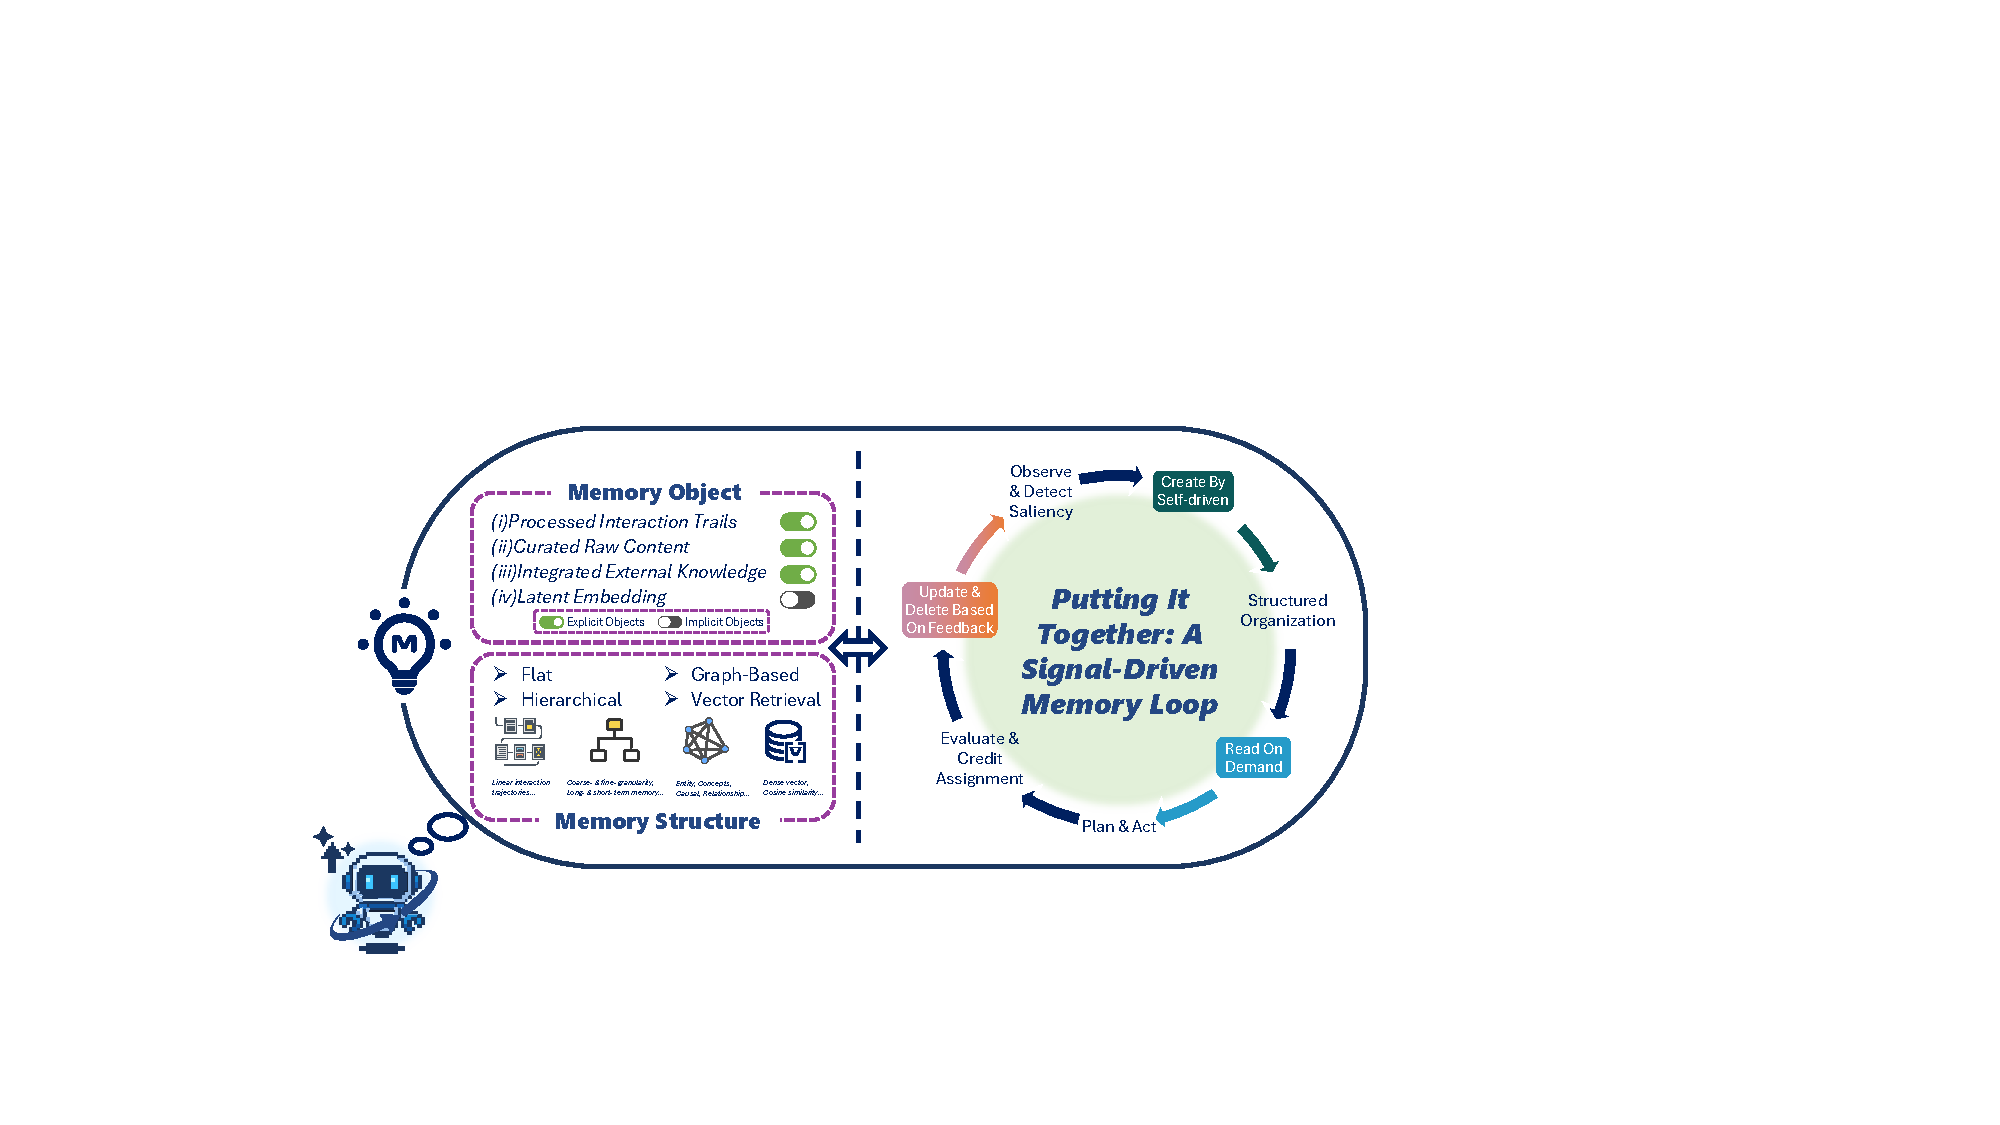
\includegraphics[width=1\linewidth]{fig/agent_memory.pdf}
    \caption{Overview of memory for self-improving agent.}
    \label{fig:agent_memory}
\end{figure*}



\subsubsection{Memory Object}
\label{sec:Memory_Object}


\makeatletter
\@ifundefined{rate}{
  \newcommand{\rate}[2]{\rate@impl{#1}{#2}}
}{
  \renewcommand{\rate}[2]{\rate@impl{#1}{#2}}
}
\newcommand{\rate@impl}[2]{
  \begingroup
  \def\filled{#1}\def\total{#2}
  \newcount\ratei \ratei=1
  \loop\ifnum\ratei<\numexpr\total+1\relax
    \ifnum\ratei>\filled
      \textcolor{black!20}{\rule{0.85ex}{0.85ex}}
    \else
      \textcolor{blue!70!black}{\rule{0.85ex}{0.85ex}}
    \fi
    \hspace{0.22ex}
    \advance\ratei by 1
  \repeat
  \endgroup
}
\makeatother


\newcommand{\bbull}{\textcolor{blue!70!black}{\raisebox{0.25ex}{\tiny$\bullet$}}\;}
\newcommand{\fbull}{\textcolor{black!55}{\raisebox{0.25ex}{\tiny$\blacktriangleright$}}\;}


\newcommand{\mini}[1]{{\scriptsize\color{black!70}#1}}

\begin{table*}[t]
\centering
\scriptsize
\setlength{\tabcolsep}{2pt} 
\renewcommand{\arraystretch}{1.25}

\caption{Memory-object scorecard (qualitative). Blue squares indicate an ordinal, literature-grounded assessment (1=low, 5=high) of typical tendencies for each memory object type, synthesized from representative system designs and reported failure analyses rather than from a single standardized benchmark.}
\vspace{0.35em}

\rowcolors{2}{lightBlue!18}{white}


\newcolumntype{L}[1]{>{\raggedright\arraybackslash}p{#1}}
\newcolumntype{R}{>{\centering\arraybackslash}m{1.05cm}} 

\begin{tabularx}{\textwidth}{
L{2.05cm}  
L{2.45cm}  
R R R R R  
X         
}
\toprule
\textbf{Object type} &
\makecell[l]{\textbf{Best-for}\\[-1pt]\textbf{persistence}} &
\textbf{Fidelity} &
\makecell[c]{\textbf{Interpre-}\\[-1pt]\textbf{tability}} &
\textbf{Compact} &
\makecell[c]{\textbf{Write}\\[-1pt]\textbf{cost}} &
\makecell[c]{\textbf{Audit-}\\[-1pt]\textbf{tability}} &
\makecell[l]{\textbf{Most common}\\[-1pt]\textbf{failure modes}} \\
\midrule


\makecell[l]{Processed\\trails} &
\makecell[l]{\bbull lessons\\[-1pt]\bbull routines\\[-1pt]\bbull summaries} &
\rate{3}{5} & \rate{5}{5} & \rate{4}{5} & \rate{3}{5} & \rate{5}{5} &
\makecell[l]{\fbull summary bias\\[-1pt]\fbull stale heuristics\\[-1pt]\fbull weak credit assignment} \\

\makecell[l]{Curated raw\\content} &
\makecell[l]{\bbull evidence\\[-1pt]\bbull exact artifacts} &
\rate{5}{5} & \rate{5}{5} & \rate{1}{5} & \rate{4}{5} & \rate{5}{5} &
\makecell[l]{\fbull context bloat\\[-1pt]\fbull retrieval noise\\[-1pt]\fbull privacy leakage surface} \\

\makecell[l]{Integrated external\\knowledge} &
\makecell[l]{\bbull shared factual state\\[-1pt]\bbull grounding} &
\rate{4}{5} & \rate{4}{5} & \rate{3}{5} & \rate{4}{5} & \rate{4}{5} &
\makecell[l]{\fbull grounding failure\\[-1pt]\fbull staleness / inconsistency\\[-1pt]\fbull tool brittleness} \\

\makecell[l]{Latent\\embeddings} &
\makecell[l]{\bbull associative carryover\\[-1pt]\bbull fast recall} &
\rate{3}{5} & \rate{1}{5} & \rate{5}{5} & \rate{2}{5} & \rate{1}{5} &
\makecell[l]{\fbull drift / contamination\\[-1pt]\fbull hard-to-debug retrieval\\[-1pt]\fbull silent corruption} \\

\bottomrule
\end{tabularx}

\label{tab:mem_object_scorecard}
\end{table*}

Recalling our formal decomposition of memory state, this subsection focuses on $\text{object}_t$, i.e., \emph{what} is stored within the agent's memory scaffold. The design of the memory object is paramount, as it directly governs storage efficiency, representation fidelity, and the capacity for cross-context knowledge transfer \citep{koley2025salmmultiagentframeworklanguage}. Moving beyond raw, exhaustive interaction trails (e.g., infinite chat histories), self-improving agents increasingly favor storing processed, high-density abstractions \citep{rasmussen2025zeptemporalknowledgegraph, deng2024humancenteredproactiveconversationalagents}. By utilizing execution feedback ($\mathcal{S}_t$) to filter or compress experiences, agents effectively mitigate context-window limitations and storage costs \citep{cao2025infiniteiclbreakinglimitcontext}. These memory objects can be fundamentally categorized into {explicit} and {implicit} representations.



\begin{itemize}[leftmargin=*]
    \item \textbf{Explicit Objects.}
    Explicit objects are human-readable and directly manipulable, which makes them the default choice when interpretability, attribution, and safety auditing are important. Their main advantage is controllability: developers can inspect, correct, and selectively expose them to the model. Their main limitation is scalability, since verbose or weakly curated memories tend to increase retrieval noise and context pressure as the memory grows.

    A first and widely used manifestation stores \textit{processed interaction trails} that compresses raw trajectories into reusable, semantically meaningful units (e.g., distilled routines, heuristics, or reflections). Driven by task success/failure signals, agents abstract generalizable strategies from experience or maintain note-like intermediate traces to support long-horizon reasoning \citep{wang2024agentworkflowmemory, ouyang2025reasoningbankscalingagentselfevolving, lanchantin2023learningreasonmemorizeselfnotes, lee2024humaninspiredreadingagentgist, long2025seeinglisteningrememberingreasoning}.


    A second manifestation retains \textit{curated raw content}. Certain scenarios require preserving exact surface details that are hard to summarize without loss (e.g., code snippets, formulas, or screenshots). Rather than storing everything, self-improving agents selectively write back only high-value artifacts validated during trial-and-error, distilling dynamic ``cheatsheets'' for future reuse \citep{zhao2024expel, suzgun2025dynamiccheatsheettesttimelearning}.

    A third manifestation integrates \textit{external knowledge}. Agents can integrate and  maintain facts from external repositories. Grounding memory in shared references rather than free-form recollection  enhances verifiability. Crucially, unlike static retrieval systems, self-improving agents utilize utility-based feedback to dynamically update, annotate, or prune these retrieved domain references (e.g., codebases or task-specific documents), thereby mitigating error propagation in downstream reasoning \citep{tran2025primeplanningretrievalintegratedmemory, zhang-etal-2024-codeagent, peng2023checkfactstryagain}.


    \item \textbf{Implicit Objects.} Implicit objects store memory in machine-native latent representations, including latent tokens, hidden states, and key--value cache augmentations. Their primary advantage is compactness and fast associative access, which makes them appealing under strict context limits or latency budgets. Their primary drawback is limited interpretability, which complicates debugging, targeted correction, and safety auditing, and can lead to representation drift when the memory is repeatedly rewritten or composed.


Recent advancements explore several mechanisms for implicit memory scaffolding without altering the base FM parameters. \textit{Generative latent memory} constructs latent sequences to enrich reasoning beyond text-based retrieval \citep{zhang2025memgenweavinggenerativelatent}. \textit{Latent state reconstruction} captures and reintegrates hidden representations to improve context retention \citep{dillon2025contextualmemoryreweavinglarge}. A related line augments the decoding process via offline coprocessors that inject latent embeddings directly into the KV cache to boost generation fidelity \citep{liu2024deliberationlatentspacedifferentiable, sun2025enhancinglatentcomputationtransformers}. Finally, maintaining self-updatable latent memory pools offers a practical compromise between persistent state tracking and strict capacity control \citep{wang2024memoryllmselfupdatablelargelanguage, wang2025mextendingmemoryllmscalable}.

\end{itemize}






\paragraph{Trade-offs.}
Explicit memory objects offer high interpretability and controllability, simplifying debugging and safety auditing, but require rigorous curation to avoid overwhelming the context budget. Among them, processed trails favor generalization, curated artifacts favor precision, and integrated external knowledge favors verifiability. Conversely, implicit memory objects provide compact, high-speed associative access and mitigate context length issues, but are difficult to inspect, correct, and are susceptible to representation drift over long horizons. We summarize these qualitative trade-offs and common failure modes in Table~\ref{tab:mem_object_scorecard}.



\newcommand{\Dfull}{\textcolor{blue!80!black}{\raisebox{0.15ex}{\large$\bullet$}}} 
\newcommand{\Dmid}{\textcolor{cyan!80}{\raisebox{0.15ex}{\large$\bullet$}}} 
\newcommand{\Dnone}{\textcolor{black!10}{\raisebox{0.15ex}{\large$\bullet$}}}


\newcommand{\Hstrut}{\rule{0pt}{3.2ex}}

\begin{table}[t]
\centering
\caption{Memory architecture and processing operators.
Checkmarks indicate the memory \emph{object} and \emph{structure} choices reported by each system.
Dots denote the relative emphasis of a mechanism as primary (\Dfull), secondary (\Dmid), or absent/unclear (\Dnone).
Processing is summarized by CRUD (Create, Read, Update, Delete).
We further characterize governance along two dimensions: \textbf{Select}, which determines what information is written and retrieved based on saliency and utility, and \textbf{Maintain}, which sustains memory quality over long horizons through consolidation, refresh, and forgetting.}
\setlength{\tabcolsep}{3pt}
\renewcommand{\arraystretch}{1.35}

\rowcolors{7}{gray!8}{white}
\resizebox{\linewidth}{!}{%
\begin{tabular}{%
  >{\raggedright\arraybackslash}m{3.0cm}
  *{12}{>{\centering\arraybackslash}m{0.92cm}}
}
\toprule
\rowcolor{tab-blue}
\multicolumn{1}{>{\centering\arraybackslash}m{3.0cm}}{%
  \multirow{2}{*}{\cellcolor{white}\centering
    \raisebox{-0.15\height}{
\includegraphics[width=1.15cm,keepaspectratio]{fig/agentmemlogo.pdf}}%
  }%
} &
\multicolumn{2}{c}{\color{white}\bfseries Object\Hstrut} &
\multicolumn{4}{c}{\color{white}\bfseries Structure\Hstrut} &
\multicolumn{4}{c}{\color{white}\bfseries Processing\Hstrut} &
\multicolumn{2}{c}{\color{white}\bfseries Governance\Hstrut} \\
\cmidrule(lr){2-3}\cmidrule(lr){4-7}\cmidrule(lr){8-11}\cmidrule(lr){12-13}

& \cellcolor{blue!12}\thead{Explicit\\Objects\Hstrut} &
  \cellcolor{blue!12}\thead{Implicit\\Objects\Hstrut} &
  \cellcolor{blue!12}\thead{Flat\Hstrut} &
  \cellcolor{blue!12}\thead{Hier.\Hstrut} &
  \cellcolor{blue!12}\thead{Graph\Hstrut} &
  \cellcolor{blue!12}\thead{Vector\\Retr.\Hstrut} &
  \cellcolor{blue!12}\thead{Create\\\tagbox{C}\kern-0.35em\Hstrut} &
  \cellcolor{blue!12}\thead{Read\\\tagbox[cyan!60!teal]{R}\Hstrut} &
  \cellcolor{blue!12}\thead{Update\\\tagbox[roseviolet]{U}\Hstrut} &
  \cellcolor{blue!12}\thead{Delete\\\tagbox[VOrange]{D}\Hstrut} &
  \cellcolor{blue!12}\thead{Select\Hstrut} &
  \cellcolor{blue!12}\thead{Maint.\Hstrut} \\
\midrule

\textbf{\hyperlink{cite.lanchantin2023learningreasonmemorizeselfnotes}{\makecell[l]{Self-Notes\\(2023)}}}
& $\checkmark$ & -- & $\checkmark$ & -- & -- & --  & \Dmid  & \Dmid  & \Dnone & \Dnone & \Dmid  & \Dnone \\

\textbf{\hyperlink{cite.park2023generativeagentsinteractivesimulacra}{\makecell[l]{Generative\\Agents (2023)}}}
& $\checkmark$ & -- & $\checkmark$ & -- & -- & $\checkmark$ & \Dmid  & \Dfull & \Dnone & \Dmid  & \Dfull & \Dmid \\

\textbf{\hyperlink{cite.guan2024richelieu}{\makecell[l]{Richelieu\\(2024)}}}
& $\checkmark$ & -- & $\checkmark$ & -- & -- & --  & \Dmid  & \Dmid  & \Dnone & \Dnone & \Dmid  & \Dnone \\

\textbf{\hyperlink{cite.suzgun2025dynamiccheatsheettesttimelearning}{\makecell[l]{DC\\(2025)}}}
& $\checkmark$ & -- & $\checkmark$ & -- & -- & --  & \Dfull & \Dmid  & \Dfull & \Dfull & \Dfull & \Dfull \\

\textbf{\hyperlink{cite.liang2025selfevolvingagentsreflectivememoryaugmented}{\makecell[l]{SAGE\\(2025)}}}
& $\checkmark$ & -- & -- & $\checkmark$ & -- & -- & \Dfull & \Dmid  & \Dfull & \Dfull & \Dmid  & \Dfull \\

\textbf{\hyperlink{cite.chhikara2025mem0buildingproductionreadyai}{\makecell[l]{Mem0\\(2025)}}}
& $\checkmark$ & -- & -- & -- & $\checkmark$ & $\checkmark$ & \Dfull & \Dfull & \Dfull & \Dfull & \Dfull & \Dfull \\

\textbf{\hyperlink{cite.salama2025meminsightautonomousmemoryaugmentation}{\makecell[l]{MemInsight\\(2025)}}}
& $\checkmark$ & -- & -- & $\checkmark$ & -- & $\checkmark$ & \Dfull & \Dfull & \Dmid  & \Dnone & \Dfull & \Dmid \\

\textbf{\hyperlink{cite.zhang2025memgenweavinggenerativelatent}{\makecell[l]{MemGen\\(2025)}}}
& -- & $\checkmark$ & $\checkmark$ & -- & -- & -- & \Dfull & \Dfull & \Dmid  & \Dnone & \Dfull & \Dnone \\

\textbf{\hyperlink{cite.zhang2025agenticcontextengineeringevolving}{\makecell[l]{ACE\\(2025)}}}
& $\checkmark$ & -- & -- & -- & -- & $\checkmark$ & \Dfull & \Dfull & \Dfull & \Dmid  & \Dmid  & \Dfull \\

\textbf{\hyperlink{cite.xu2025amemagenticmemoryllm}{\makecell[l]{A-MEM\\(2025)}}}
& $\checkmark$ & -- & -- & -- & $\checkmark$ & $\checkmark$ & \Dfull & \Dfull & \Dfull & \Dnone & \Dfull & \Dfull \\

\textbf{\hyperlink{cite.wang2024agentworkflowmemory}{\makecell[l]{AWM\\(2024)}}}
& $\checkmark$ & -- & -- & $\checkmark$ & -- & -- & \Dfull & \Dmid  & \Dmid  & \Dnone & \Dmid  & \Dnone \\

\textbf{\hyperlink{cite.ouyang2025reasoningbankscalingagentselfevolving}{\makecell[l]{Reasoning\\Bank (2025)}}}
& $\checkmark$ & -- & -- & -- & -- & $\checkmark$ & \Dfull & \Dmid  & \Dmid  & \Dnone & \Dmid  & \Dnone \\

\textbf{\hyperlink{cite.lee2024humaninspiredreadingagentgist}{\makecell[l]{ReadAgent\\(2024)}}}
& $\checkmark$ & -- & $\checkmark$ & -- & -- & -- & \Dmid  & \Dfull & \Dnone & \Dnone & \Dmid  & \Dnone \\

\textbf{\hyperlink{cite.long2025seeinglisteningrememberingreasoning}{\makecell[l]{M3-Agent\\(2025)}}}
& $\checkmark$ & -- & -- & $\checkmark$ & -- & -- & \Dmid  & \Dmid  & \Dmid  & \Dmid  & \Dmid  & \Dmid \\

\textbf{\hyperlink{cite.zhao2024expel}{\makecell[l]{ExpeL\\(2024)}}}
& $\checkmark$ & -- & -- & -- & -- & $\checkmark$ & \Dfull & \Dmid  & \Dmid  & \Dnone & \Dfull & \Dmid \\

\textbf{\hyperlink{cite.tran2025primeplanningretrievalintegratedmemory}{\makecell[l]{PRIME\\(2025)}}}
& $\checkmark$ & -- & -- & -- & -- & $\checkmark$ & \Dnone & \Dfull & \Dnone & \Dnone & \Dfull & \Dnone \\

\textbf{\hyperlink{cite.zhang-etal-2024-codeagent}{\makecell[l]{CodeAgent\\(2024)}}}
& $\checkmark$ & -- & -- & -- & -- & $\checkmark$ & \Dnone & \Dfull & \Dnone & \Dnone & \Dfull & \Dnone \\

\textbf{\hyperlink{cite.dillon2025contextualmemoryreweavinglarge}{\makecell[l]{CMR\\(2025)}}}
& -- & $\checkmark$ & -- & $\checkmark$ & -- & -- & \Dfull & \Dfull & \Dfull & \Dnone & \Dmid  & \Dfull \\

\textbf{\hyperlink{cite.wang2024memoryllmselfupdatablelargelanguage}{\makecell[l]{MemoryLLM\\(2024)}}}
& -- & $\checkmark$ & $\checkmark$ & -- & -- & -- & \Dfull & \Dfull & \Dfull & \Dnone & \Dmid  & \Dfull \\

\textbf{\hyperlink{cite.wang2025mextendingmemoryllmscalable}{\makecell[l]{M+\\(2025)}}}
& -- & $\checkmark$ & $\checkmark$ & -- & -- & -- & \Dfull & \Dfull & \Dfull & \Dnone & \Dmid  & \Dfull \\

\textbf{\hyperlink{cite.sun2025hierarchicalmemoryhighefficiencylongterm}{\makecell[l]{H-MEM\\(2025)}}}
& $\checkmark$ & -- & -- & $\checkmark$ & -- & -- & \Dmid  & \Dfull & \Dfull & \Dmid  & \Dmid  & \Dmid \\

\textbf{\hyperlink{cite.koley2025salmmultiagentframeworklanguage}{\makecell[l]{SALM\\(2025)}}}
& $\checkmark$ & -- & -- & $\checkmark$ & -- & -- & \Dmid  & \Dfull & \Dmid  & \Dmid  & \Dmid  & \Dmid \\

\textbf{\hyperlink{cite.cheng2022xmemlongtermvideoobject}{\makecell[l]{XMem\\(2022)}}}
& -- & $\checkmark$ & -- & $\checkmark$ & -- & -- & \Dnone & \Dfull & \Dmid  & \Dnone & \Dnone & \Dnone \\

\textbf{\hyperlink{cite.song2024moviechatdensetokensparse}{\makecell[l]{MovieChat\\(2024)}}}
& -- & $\checkmark$ & -- & $\checkmark$ & -- & $\checkmark$ & \Dmid  & \Dfull & \Dmid  & \Dnone & \Dnone & \Dnone \\

\textbf{\hyperlink{cite.helmi2025decentralizingaimemoryshimi}{\makecell[l]{SHIMI\\(2025)}}}
& $\checkmark$ & -- & -- & $\checkmark$ & $\checkmark$ & -- & \Dmid  & \Dfull & \Dmid  & \Dmid  & \Dfull & \Dmid \\

\bottomrule
\end{tabular}%
}
\label{tab:memory_architecture}
\end{table}


\subsubsection{Memory Structure}
\label{sec:Memory_Structure}

Building upon the definition of memory objects ($\text{object}_t$), the memory structure ($\text{structure}_t$) specifies the organizational schema and relational topology through which these objects are indexed, linked, and retrieved. For self-improving agents operating in complex, dynamic environments, an adaptive memory structure acts as more than a passive database; it actively empowers the agent to consolidate long-horizon experiences, resolve context fragmentation, and perform robust relational reasoning \citep{zeng2024structuralmemoryllmagents}. Consequently, how this structure is designed and updated directly dictates the agent's ability to scale its cognitive baseline efficiently. Prevailing structural paradigms can be broadly categorized into the following  forms, each offering distinct trade-offs in scalability, expressiveness, and retrieval latency:


\begin{itemize}[leftmargin=*]
    \item \textbf{Flat Structure.}     Flat memories store entries in strict temporal order. This append-only design makes writing computationally cheap and  preserves the causal narrative of interaction. This topology is particularly advantageous for self-improving loops that rely on trajectory replay, as it maintains the unadulterated context necessary to diagnose failures ($\mathcal{S}_t$) and reproduce successful behaviors. The primary cost is retrieval scalability. As the stream expands, recall becomes overly dependent on truncation heuristics or coarse filtering. Consequently, agents often suffer from recency bias—surfacing recent but irrelevant interactions while missing older, decisive evidence. Furthermore, lacking inherent support for abstraction, flat structures tend to accumulate redundant low-level traces, exacerbating context pressure over long horizons \citep{antony2024causal, sun2025hierarchicalmemoryhighefficiencylongterm}. Representative systems operationalize this design by augmenting chronological logs with lightweight indexing. For instance, SCM maintains a temporal memory stream enriched with summaries and embeddings, bridging basic semantic search with chronological access \citep{wang2025scmenhancinglargelanguage}. Similarly, frameworks like Self-Notes write transient insights directly inline during long-context reasoning. This keeps the memory  aligned with the evolving cognitive state, allowing for immediate, feedback-driven course corrections while preserving the chronological flow of thought \citep{lanchantin2023learningreasonmemorizeselfnotes}.

\item \textbf{Hierarchical Structure.}
    Hierarchical memories organize objects across multiple abstraction levels, addressing a central bottleneck in self-improving agents: the need to compress long histories into stable, reusable knowledge while preserving interaction-level details. By allocating high-level summaries, mid-level plans, and low-level traces into distinct layers, this topology reduces retrieval noise and supports long-horizon coherence. However, the primary risk is structural brittleness. If the induced taxonomy misaligns with the task, strict hierarchies can fragment evidence and hinder cross-cutting retrieval, which severely impedes the agent's ability to recombine diverse experiences for continual improvement. Recent systems instantiate this hierarchy through different organizational lenses. For \textit{task-oriented} abstraction, MobileGPT employs a goal-to-subtask-to-action hierarchy for GUI tasks, supporting both plan reuse and fine-grained execution recall~\citep{lee2024exploreselectderiverecall}. For \textit{semantic} abstraction, H-MEM~\citep{sun2025hierarchicalmemoryhighefficiencylongterm} and SHIMI~\citep{helmi2025decentralizingaimemoryshimi} construct multi-level semantic nodes, enabling coarse-to-fine retrieval and top-down traversal from abstract intents to specific entities. Alternatively, SALM approaches hierarchy via \textit{tiered storage patterns} (short-term, long-term) to separate active context maintenance from durable reuse~\citep{koley2025salmmultiagentframeworklanguage}. Besides, similar principles extend to multimodal domains, where agents separate transient perceptual buffers from persistent representations for long-video understanding, drawing inspiration from classical human memory models~\citep{cheng2022xmemlongtermvideoobject, song2024moviechatdensetokensparse, atkinson1968human}.

    \item \textbf{Graph-Based Structure.} Graph memories represent objects as nodes linked by semantic, temporal, or causal edges, aligning naturally with the need for self-improving agents to generalize across continuous interactions. By explicitly encoding relations, this topology replaces recency-based recall with retrieval by association. It enables multi-hop evidence aggregation that flat streams or strict trees struggle to support, which is vital when agents must attribute failures to latent dependencies, track evolving entity states, or reuse abstracted insights. However, the primary trade-off is maintenance complexity. Continuous graph construction, edge updating, and conflict resolution introduce significant computational overhead and risk structural drift as the agent repeatedly edits its own memory.

       Recent literature explores this paradigm through different relational lenses. For {semantic and conversational} tracking, systems like Mem0~\citep{chhikara2025mem0buildingproductionreadyai} and SGMem~\citep{wu2025sgmemsentencegraphmemory} parse dialogues into fact- or sentence-level graphs to support highly structured recall. To support {temporal  and causal} reasoning, Zep provides a temporal-aware knowledge graph for continuous belief revision~\citep{rasmussen2025zeptemporalknowledgegraph}, while CausalRAG leverages explicit causal edges to prevent spurious correlations from contaminating the self-improvement loop~\citep{wang2025causalragintegratingcausalgraphs}. Some approaches even blend topologies; for instance, G-Memory introduces a {hybrid hierarchical graph} to separate reusable insights from fine-grained logs in multi-agent settings~\citep{zhang2025gmemorytracinghierarchicalmemory}. Beyond text, explicit graph structures are similarly crucial for multimodal agents—such as GraphVideoAgent and Scene-MMKG—where maintaining spatial-temporal state transitions and entity interactions is essential for grounded reasoning~\citep{10.1145/3746027.3755537, 10531671}.


    \item \textbf{Vector Retrieval Structure.}
    Vector-based memory indexes objects by dense embeddings and retrieves by similarity, which makes it a strong default when an agent must recall semantically related interactions under natural language queries. For self-improving agents, it serves as the primary engine for episodic recall and large-scale knowledge assimilation, supporting continual expansion without a hand-crafted schema.      
    Its dominant failure mode is misalignment between similarity and usefulness. The nearest neighbors under an embedding metric may be topically similar yet decision-irrelevant, and this retrieval noise can systematically bias the agent's subsequent learning updates.  As a result, self-improving systems often augment vector retrieval with re-ranking, hybrid signals, or adaptive controllers that dynamically gate the retrieval process.


    Building upon the classic RAG pipeline~\citep{lewis2021retrievalaugmentedgenerationknowledgeintensivenlp}, Agentic RAG integrates autonomous control over retrieval to manage dynamic episodic memories~\citep{ravuru2024agenticretrievalaugmentedgenerationtime, singh2025agenticretrievalaugmentedgenerationsurvey}. To mitigate the similarity-usefulness misalignment, systems explore various optimizations: \textit{hybrid heuristics}, such as Generative Agents combining dense relevance with recency and importance~\citep{park2023generativeagentsinteractivesimulacra}; and \textit{adaptive representations}, where RMM introduces differentiable ranking to improve recall under long-term dialogues~\citep{tan2025prospectretrospectreflectivememory}. For domain-specific trajectory reuse, systems like MemoryBank~\citep{zhong2024memorybank} and CTIM-Rover~\citep{lindenbauer2025knowledgenoisectimroverpitfalls} index episodic segments to robustly fetch past successes, whereas MIRIX routes queries across multiple specialized sub-stores to overcome the limits of a flat index~\citep{wang2025mirixmultiagentmemoryllmbased}. Finally, this vector-based topology readily accommodates multimodal experiences, enabling embodied agents like MrSteve to retrieve relevant past video frames for exploration~\citep{park2025mrsteveinstructionfollowingagentsminecraft}.

\end{itemize}

\subsubsection{Memory Processing}
\label{sec:Memory_Processing}
Given the memory state $m_t := (\text{object}_t,\text{structure}_t)$, memory processing refers to the family of signal-driven operations that act on $m_t$ throughout an agent's lifetime.  Formally, we view memory improvement as $m_{t+1} = \text{IMPROVE}_m(m_t; \mathcal{S}_t)$. Unlike traditional agents that rely on static, hard-coded indexing, self-improving agents use the learning signal $\mathcal{S}_t$ (e.g., task outcomes, utility, or internal critiques) to dynamically adjust what to write, how to retrieve, and when to forget \citep{xu2025sedmscalableselfevolvingdistributed, liang2025selfevolvingagentsreflectivememoryaugmented}. Concretely, we instantiate $\text{IMPROVE}_m$ as an adaptive CRUD (Create, Read, Update, Delete) operation family: 


\paragraph{\tagbox{C}} Rather than appending raw logs exhaustively, memory creation is a selective distillation process guided by $\mathcal{S}_t$. Recent systems typically implement this through three recurring patterns: (1) \emph{Semantic compression}, which transforms raw interactions into structured metadata, summaries, or reusable schemas for efficient indexing~\citep{salama2025meminsightautonomousmemoryaugmentation, wang2024agentworkflowmemory, ouyang2025reasoningbankscalingagentselfevolving}; (2) \emph{Context-aware discrete decisions} (e.g., add, update, delete, or no-op), conditioned on retrieved neighbors to prevent redundant or conflicting entries~\citep{chhikara2025mem0buildingproductionreadyai, xu2025amemagenticmemoryllm}; and (3) \emph{Controlled boundary insertion}, which dynamically optimizes the write policy for downstream utility closer to generation time~\citep{zhang2025memgenweavinggenerativelatent}. Across all designs, creation is bounded by a trade-off: over-writing inflates retrieval noise, whereas under-writing sacrifices long-term capability.



\paragraph{\tagbox[cyan!60!teal]{R}}  Memory reading dictates the quality of an agent's downstream reasoning. To maintain precision as the memory bank scales, self-improving systems typically employ four key mechanisms: (1) \emph{Hybrid heuristics}, which blend semantic relevance with recency and importance scores to stabilize recall~\citep{park2023generativeagentsinteractivesimulacra}; (2) \emph{Structure-aware retrieval}, which performs coarse-to-fine traversal over hierarchical or graph topologies to isolate reusable abstractions from low-level traces~\citep{zhang2025gmemorytracinghierarchicalmemory}; (3) \emph{Retrieval gating}, which dynamically decides whether to query memory and how much context is sufficient, thereby optimizing token cost and minimizing distraction~\citep{wang2025scmenhancinglargelanguage}; and (4) \emph{Retrieval-driven adaptation}, where historical trajectories are fetched as actionable cases to guide behavior without requiring parametric model updates~\citep{zhou2025mementofinetuningllmagents}. Ultimately, ineffective reading policies will hinder performance: retrieving irrelevant noise or missing critical details will directly cause subsequent planning and execution to fail.



\paragraph{\tagbox[roseviolet]{U}} Memory updating is the primary mechanism for self-correction and knowledge evolution. Guided by feedback ($\mathcal{S}_t$), agents typically implement updates through four operational patterns: (1) \emph{Scheduled review and attenuation}, which periodically strengthens high-utility items and decays obsolete ones to stabilize memory growth~\citep{liang2025selfevolvingagentsreflectivememoryaugmented}; (2) \emph{Local refresh}, which dynamically updates topological neighbors during new insertions to maintain contextual consistency~\citep{xu2025amemagenticmemoryllm}; (3) \emph{Iterative distillation}, which synthesizes repeated successes into compact, reusable abstractions via continuous selection and replacement~\citep{suzgun2025dynamiccheatsheettesttimelearning, zhang2025agenticcontextengineeringevolving}; and (4) \emph{Offline aggregation}, which shifts computationally expensive compression away from the online execution loop while preserving recall quality~\citep{fang2025lightmemlightweightefficientmemoryaugmented}. Without effective update policies, agents suffer from memory decay: outdated facts remain, knowledge structures break down, and improper merging erases important details.
 

\paragraph{\tagbox[VOrange]{D}} Memory deletion acts as a systematic noise reduction and resource optimization mechanism. Guided by signal ($\mathcal{S}_t$), agents dynamically identify and remove obsolete or redundant entries through three main patterns: (1) \emph{Multi-stage pruning}, which filters low-value items at write time and periodically clears entries based on access frequency and relevance~\citep{zhang2025mlcagentcognitivemodelbased}; (2) \emph{Consensus-based eviction}, which uses collaborative voting in distributed setups to prevent the accidental deletion of critical shared knowledge~\citep{bach2025pbftbackedsemanticvotingmultiagent}; and (3) \emph{Tiered eviction}, which applies operating-system-inspired rules across different memory layers to bound size while preserving long-term consistency~\citep{kang2025memory}. Improper deletion policies create a direct dilemma: over-pruning loses critical knowledge, while under-pruning floods the system with outdated noise and slows down retrieval.


\paragraph{Putting it together: a signal-driven memory loop.} The dimensions of memory objects, structure, and processing culminate in a unified, signal-driven lifecycle (Figure~\ref{fig:agent_memory}). This loop proceeds in a continuous cycle: (i) Observe \textit{\&} Detect saliency from new interactions; (ii) Create compact objects; (iii) Organize them into the chosen topological structure; (iv) Read on demand via adaptive retrieval; (v) Plan \textit{\&} Act based on fetched context; (vi) Evaluate outcomes to derive the learning signal $\mathcal{S}_t$; and (vii) Update/Delete entries to consolidate high-value knowledge and prune noise. Together, these stages elevate memory from a passive cache to a self-governing engine that sustains open-ended autonomy.


\begin{ttcolorbox}[Takeaway]
The Self-Improvement Memory Loop transforms the conceptual questions of memory management into an actionable, signal-driven framework. By unifying memory writing, structural organization, adaptive retrieval, and feedback-based pruning, this continuous lifecycle effectively elevates memory from a static cache to a scalable engine for self-improvement.
\end{ttcolorbox}


\subsection{Tool}
\label{sec:Tool}

Basic agents have been constrained by their reliance on static, manually curated toolkits, lacking the autonomy to adapt, discover, or integrate new resources when confronted with novel challenges \citep{shapiro2023conceptual, zhang2025largelanguagemodelbrainedgui, sang2025pipelinessurveyparadigmshift, huang2025surveyfoundationmodelpoweredrecommender}. The transition from a basic executor to a genuinely self-improving agent necessitates a shift away from simple, pre-defined tool use toward \textit{Tool Governance Metacognition}. This dynamic paradigm empowers the agent to autonomously reason about the necessity, utility, and reliability of its tools, thereby continually advancing its capability boundaries rather than merely operating within them \citep{liu2025trulyselfimprovingagentsrequire, yin2024g}.

\begin{wrapfigure}{r}{0.37\textwidth}
  \vspace{-\intextsep}        
  \centering
  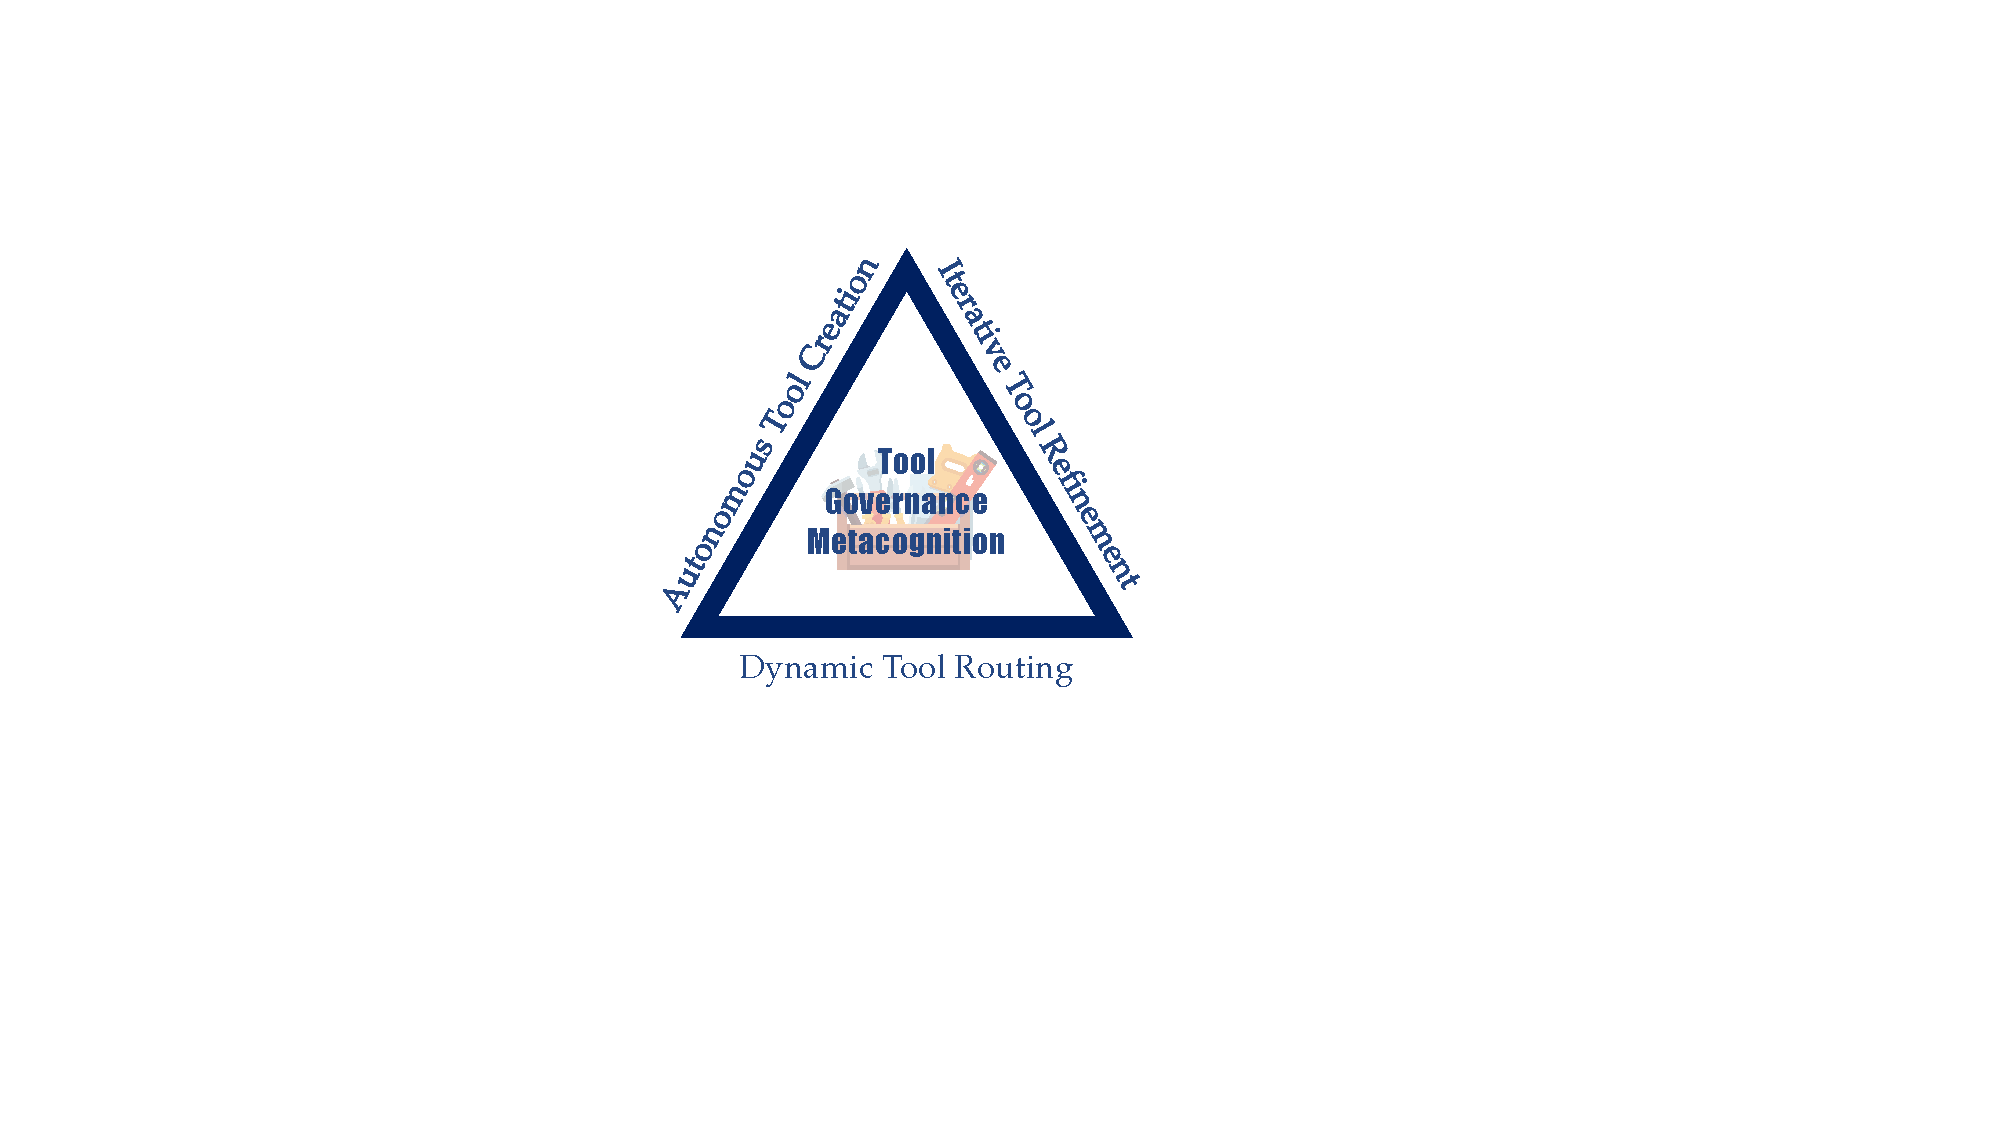
\includegraphics[width=\linewidth]{fig/fig-tool.pdf}
  \caption{Tool Governance Metacognition.}
  \label{fig:agent_tool}
  \vspace{-1pt}             
\end{wrapfigure}

Formally, tool-based improvement can be written as
\begin{equation}
\mathcal{T}_{t+1}=\IMPROVE_{\mathcal{T}}(\mathcal{T}_t;\mathcal{S}_t),
\end{equation}
where $\mathcal{S}_t$ is the learning signal produced by tool governance metacognition. This metacognition represents the architectural shift essential for a self-improving agent, establishing a dynamic and self-directed mechanism for managing its operational tools \citep{wang2025theoryagentstoolusedecisionmakers}. It is instantiated through three core dimensions: Dynamic Tool Routing, which orchestrates the efficient selection and combination of tools from a growing pool; Iterative Tool Refinement, which adapts and debugs existing instruments to overcome execution failures or environmental shifts; and Autonomous Tool Creation, which invents novel tools to fundamentally expand the agent's capability boundaries. This governance structure moves tool use from a static look-up process to a generative, self-improving cycle.


\subsubsection{Dynamic Tool Routing}
\label{sec:Dynamic_Tool_Routing}

Dynamic tool routing concerns how an agent selects, sequences, and coordinates tools in a heterogeneous environment. As tool pools grow, routing becomes a primary bottleneck for self-improvement. A large tool set increases coverage but also increases error modes, including misrouting, compounding execution failures, and wasted compute. Routing methods therefore trade off coverage, reliability, and decision cost. Most existing systems can be understood through three routing paradigms, distinguished by what they treat as the ``retrieval unit'' and how they incorporate feedback over time.



\paragraph{\textcolor{Plum}{Retrieval- and graph-based routing.}}
Systems in this paradigm tackle the routing bottleneck by optimizing either the retrieval space or the representation of dependencies. To optimize the retrieval space and maintain scalability, systems dynamically manage the granularity and scope of the tool pool. For instance, while MemTool prevents routing degradation by actively pruning the tool set into a lightweight operational memory~\citep{lumer2025memtooloptimizingshorttermmemory}, TAR expands the retrieval unit itself, dynamically routing between atomic APIs and entire competent agents to handle higher-level tasks~\citep{lumer2025tooltoagentretrievalbridgingtools}. Crucially for self-improvement, this retrieval process is not static; it evolves by leveraging past successes as a learning signal. Systems like VOYAGER and MetaAgent index reusable tool-use trajectories into procedural memory, allowing the routing policy to continuously refine itself based on structural knowledge from prior executions~\citep{wang2023voyageropenendedembodiedagent, qian2025metaagentselfevolvingagenttool}. Conversely, to address the compositionality limitation of flat retrieval, recent works encode tool transitions as topological structures. Rather than one-shot relevance, systems like ToolNet and OrchDAG model tool dependencies as directed graphs, enabling routing that accounts for multi-step feasibility and preconditions~\citep{liu2024toolnetconnectinglargelanguage, lu2025orchdagcomplextoolorchestration}. Building on this, MassTool combines learned semantic matching with these graph structures, achieving high-precision navigation even within massive and complex tool topologies~\citep{lin2025masstoolmultitasksearchbasedtool}.


\paragraph{\textcolor{Plum}{Policy-learning routing.}} Policy-learning routing internalizes tool choice as sequential decision making. Instead of retrieving a tool from an external index, the agent learns invocation behavior from training signals, which can improve robustness in multi-turn settings where success depends on state, history, and error recovery. The main trade-off is data and feedback. Learned routing can overfit to training environments and can be brittle when tool interfaces or distributions drift. To establish a reliable routing baseline, systems like AUTOACT, MCP-Flow, Tool-Star, and DeepEyesV2 bootstrap policies through supervised fine-tuning on synthetic or mined trajectories~\citep{qiao2024autoactautomaticagentlearning, wang2025mcpflowfacilitatingllmagents, dong2025tool, hong2025deepeyesv2agenticmultimodalmodel}. However, to continually improve long-horizon behavior, routing policies must transcend static supervision. Works like AGENTFLOW and SPORT achieve this by applying sparse rewards or preference signals to shape planning and exploration, while AutoTIR and DeepAgent explicitly align tool selection with multi-objective compliance and action-level attribution~\citep{li2025intheflowagenticoptimizationeffective, li2025iterative, wei2025autotirautonomoustoolsintegrated, li2025deepagentgeneralreasoningagent}. Pushing this paradigm to its limit, ToolGen collapses retrieval, selection, and invocation into a single generative process via tool-token unification. While this elegantly reduces pipeline complexity, it places a heavy burden on the learned policy to remain calibrated under distribution shifts~\citep{wang2025toolgenunifiedtoolretrieval}.


\paragraph{\textcolor{Plum}{Proactive and interactive routing.}}
A third paradigm treats routing as an interactive process rather than a one-shot decision. This perspective is motivated by two recurring failure sources in self-improving agents. First, user intent is often underspecified, and misrouting can be avoided by clarification. Second, execution failures are common, and routing must support local repair without restarting the entire plan. Proactive routing therefore trades additional interaction and compute for higher reliability. Rather than failing passively, these systems embed metacognitive interventions to handle uncertainty. When confronting underspecified intents or functional gaps, agents like MCP-Zero and ASKTOACT proactively initiate tool discovery or prompt for clarification, transforming ambiguity into a learning signal for self-correction~\citep{fei2025mcpzeroactivetooldiscovery, zhang2025asktoactenhancingllmstool}. Conversely, when facing execution failures, dynamic repair becomes essential. Tool-Planner facilitates this by clustering tools into interchangeable kits, enabling localized, API-level repair without the prohibitive cost of global replanning~\citep{liu2025toolplannertaskplanningclusters}. Similarly, ToolACE-R dynamically calibrates its revision effort based on task difficulty, balancing routing reliability against practical compute budgets in real-world deployments~\citep{zeng2025toolacermodelawareiterativetraining}.

\subsubsection{Iterative Tool Refinement}
\label{sec:Iterative_Tool_Refinement}

Iterative tool refinement is the mechanism by which agents turn fragile programs into dependable skills. It is central to self-improvement because tool errors are not merely execution-time failures. If unreliable tools are stored and reused, they can corrupt the agent's future behavior through repeated retrieval and compounding errors. Refinement therefore serves both as debugging and as a gatekeeping process that controls what enters the structural skill repository~\citep{11185878, dolcetti2025helpingllmsimprovecode, petrovic2025surveygenaiautomotivesoftware}.


A canonical refinement loop alternates between generation, execution, and revision. VOYAGER establishes this baseline by executing generated code, capturing error traces and environment feedback as learning signals ($\mathcal{S}_t$), and feeding them back into subsequent revisions until a verifier confirms success~\citep{wang2023voyageropenendedembodiedagent}. Building on this foundation, recent systems strengthen the refinement process across three dimensions: (1) Critique Specialization. To enhance diagnostic accuracy, systems move beyond generic self-reflection. For instance, STELLA deploys a dedicated critic agent to assess intermediate results and provide targeted feedback, mitigating the tendency of monolithic models to overlook domain-specific failure modes~\citep{jin2025stellaselfevolvingllmagent}. (2) API Abstraction. Rather than merely revising raw action traces, several works focus on abstracting robust subroutines. SkillWeaver distills interactions into reusable web tools refined through execution feedback~\citep{zheng2025skillweaverwebagentsselfimprove}, while PyVision dynamically refines Python programs to stabilize multimodal tool use against noisy perception~\citep{zhao2025pyvisionagenticvisiondynamic}. This abstraction significantly improves skill transfer across tasks. (3) Interface Alignment. Addressing the semantic gap between agents and tools, systems like DRAFT iteratively refine tool documentation rather than the underlying code. This targets the critical observation that many execution failures stem from mismatches between natural language instructions and tool affordances, rather than from flawed  implementations~\citep{qu2025explorationmasteryenablingllms}.


\subsubsection{Autonomous Tool Creation}
\label{sec:Autonomous_Tool_Creation}

Autonomous tool creation expands the agent's capability boundary by synthesizing new executable functions when existing tools are insufficient. For self-improving agents, creation is most valuable when it converts one-off problem solving into reusable procedural knowledge. It also introduces its own risks. Newly created tools must be validated, documented, and integrated without destabilizing routing policies, otherwise tool growth can increase brittleness rather than autonomy~\citep{gao2025surveyselfevolvingagentspath, qiu2025alitageneralistagentenabling}.

Existing systems approach this challenge by advancing tool creation across three dimensions: (1) Synthesis Triggers. Tool creation can be driven either by immediate needs or open-ended curiosity. While systems like ATLASS and PyVision emphasize on-demand invention—synthesizing and refining tools  when current retrieved APIs fail~\citep{haque2025advancedtoollearningselection, zhao2025pyvisionagenticvisiondynamic}, agents like FRIDAY and STELLA shift toward self-directed exploration. They autonomously propose curricula or discover domain-specific resources (e.g., bioinformatics) to proactively accumulate tools outside a fixed task list~\citep{wu2024oscopilotgeneralistcomputeragents, jin2025stellaselfevolvingllmagent}. (2) Lifecycle Automation. Synthesizing raw code is only the first step; rendering it executable is the actual bottleneck. TOOLMAKER addresses this by automating the end-to-end tool lifecycle, extracting logic from scientific papers, installing dependencies, debugging in a closed loop, and producing robust callable interfaces~\citep{wölflein2025llmagentsmakingagent}. This transforms abstract function generation into tangible deployability~\citep{cai2024largelanguagemodelstool, yuan2024craftcustomizingllmscreating, qian2024creatortoolcreationdisentangling}. (3) Standardized Integration. To ensure that explosive tool growth does not destabilize existing routing policies, recent systems adopt protocol-driven architectures. Frameworks like Alita and Code2MCP automate the conversion of code repositories into standardized services via the Model Context Protocol (MCP)~\citep{qiu2025alitageneralistagentenabling, qiu2025alitagselfevolvinggenerativeagent, ouyang2025code2mcptransformingcoderepositories}. Similarly, AgentOrchestra enforces a rigorous pipeline of intent parsing, validation, and formal registration before a new tool enters the active pool~\citep{zhang2025agentorchestraorchestratinghierarchicalmultiagent}. This ensures that autonomous creation remains fully compatible with the agent's broader governance and retrieval constraints.



\begin{ttcolorbox}[Takeaway]
Based on the Tool Governance Metacognition framework, self-improving agents evolve tool usage into a growth-oriented architecture with dynamic routing, iterative refinement, and autonomous creation capabilities. This architecture transforms the system from a static toolkit into a dynamic skill repository with sustainably expandable capabilities.
\end{ttcolorbox}


\subsection{Full Scaffolding}
\label{sec:Full_Scaffolding}


Full scaffolding self-improvement represents the deepest level of architectural intervention. Rather than merely tuning isolated components (e.g., prompts, tools, or memory), the agent treats its entire operational logic and codebase as a mutable substrate, enabling fundamental structural reorganization. Formally, recalling the agent state $\mathcal{A}_t=(\theta_t,\Sigma_t)$, full scaffolding improvement corresponds to the most general \emph{scaffolding-only} transition:
\begin{equation}
\qquad \Sigma_{t+1}=\IMPROVE_{\Sigma}(\Sigma_t;\mathcal{S}_t),
\end{equation}
where $\mathcal{S}_t$ denotes the learning signal extracted from the agent's own execution traces and evaluations (e.g., task success/failure, unit tests, self-critique, cost signals).
Crucially, unlike settings with a fixed external meta-optimizer, the improvement procedure is itself implemented within the current scaffolding, making the update \emph{self-referential}:
\begin{equation}
\Sigma_{t+1} = \mathcal{I}_{\Sigma_t}(\Sigma_t;\mathcal{S}_t),
\end{equation}
where $\mathcal{I}_{\Sigma_t}$ highlights that the improver can evolve together with the agent it improves. In principle, these self-referential loops can discover unanticipated update strategies and enhance the agent's intrinsic evolvability~\citep{zhang2025darwingodelmachineopenended, gerhart2007theory, hendrikse2007evolvability, dawkins2019evolution}. While fully open-ended recursive self-improvement remains a grand challenge, current systems successfully operationalize this concept within defined objectives, benchmarks, and safety protocols.


\begin{figure*}[ht]
    \centering
    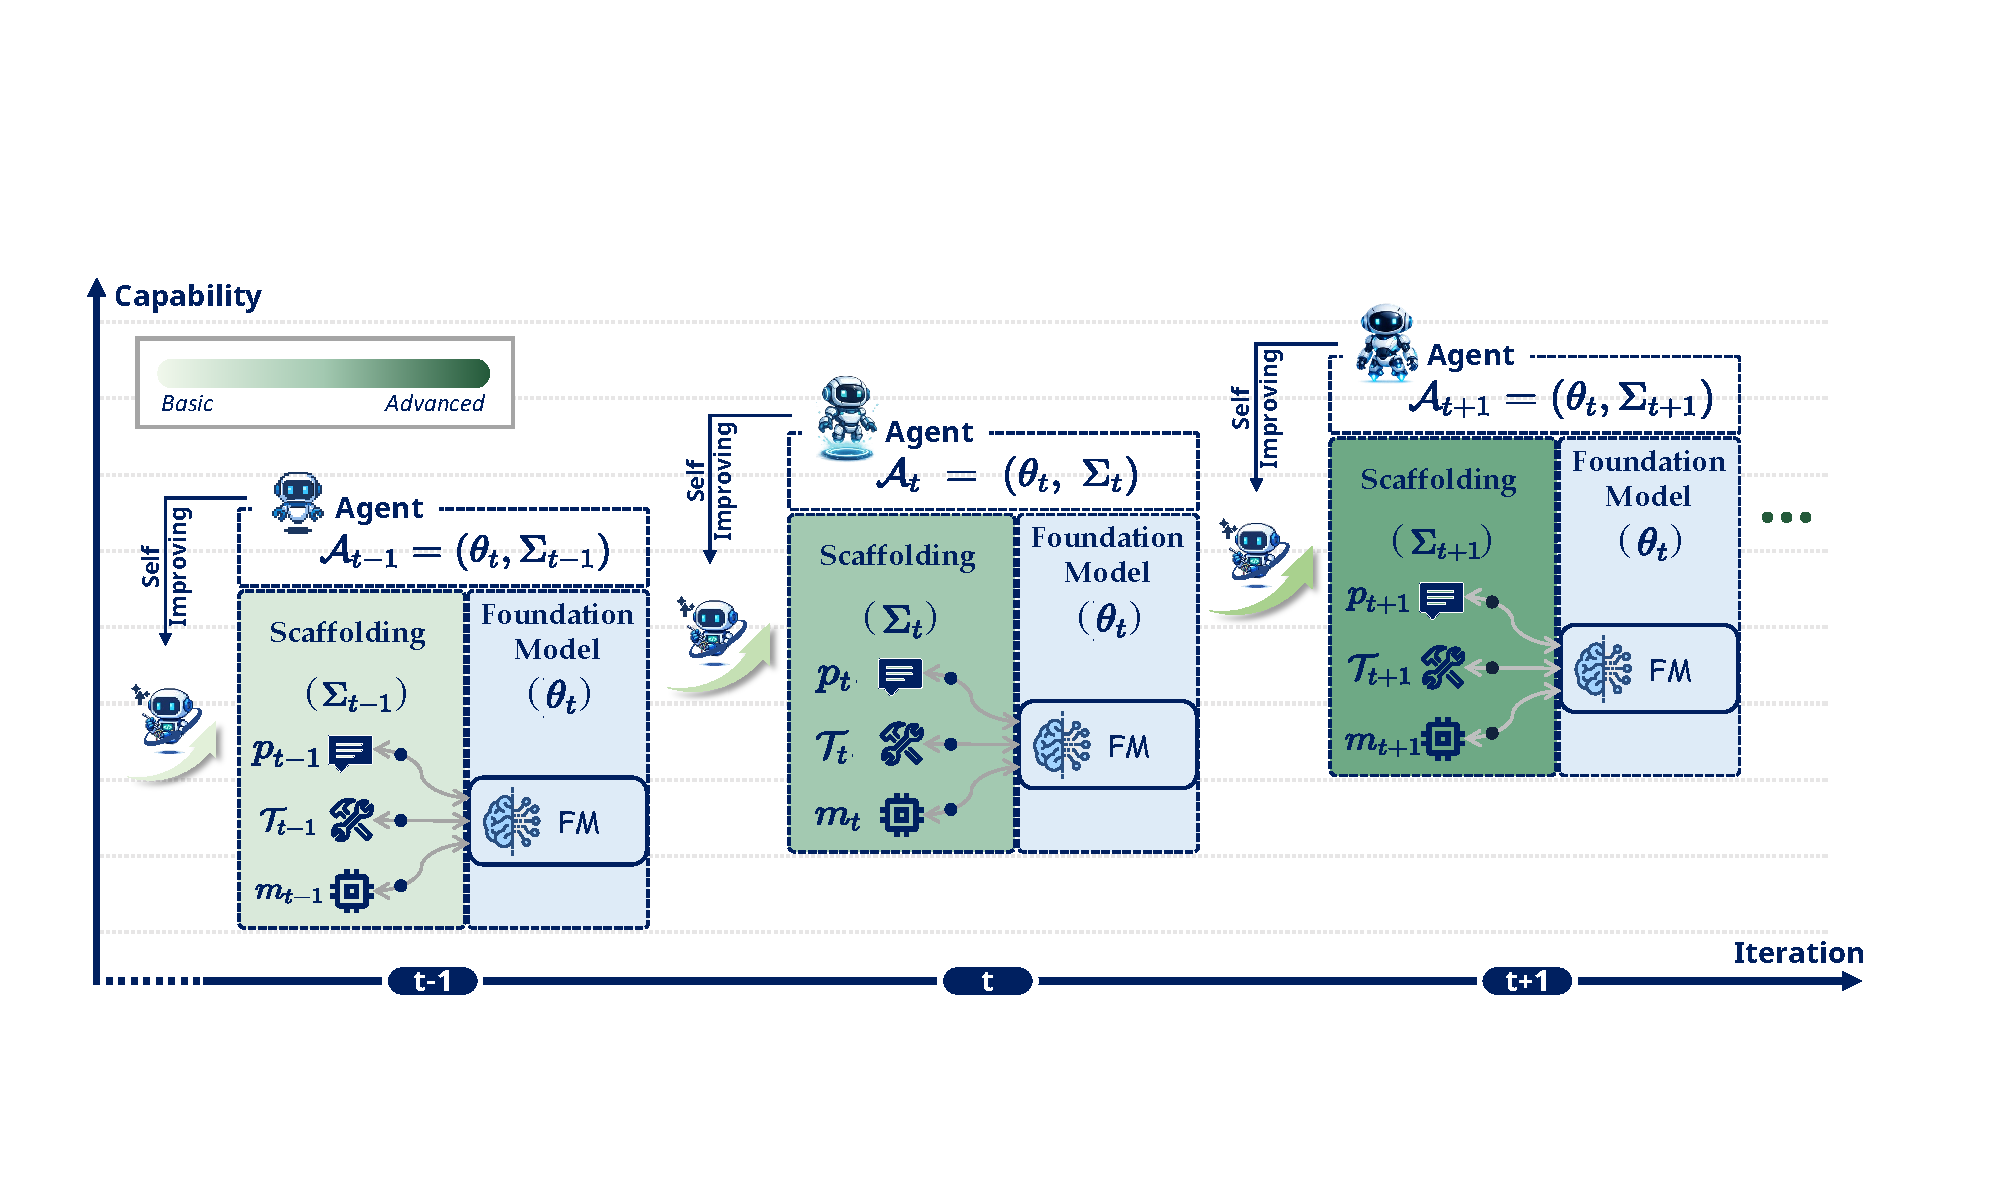
\includegraphics[width=1\linewidth]{fig/full_sacffolding.pdf}
    \caption{Full scaffolding self-improvement across iterations.}
    \label{fig:full_sacffolding}
\end{figure*}

Within this paradigm, agents' scaffolding is typically represented as conventional computer programs with mild constraints. {Formally,} let $\langle \Sigma_t \rangle$ denote a serializable encoding of the program that implements the agent, and let $exec(\cdot)$ denote execution in an environment (e.g., an interpreter, compiler, and sandbox).
A full-scaffolding update can be viewed as producing a candidate program via executing the current agent-as-improver on its own code:
\begin{equation}
\langle \tilde{\Sigma}_{t+1} \rangle = exec(\langle \Sigma_t \rangle;\mathcal{S}_t),
\end{equation}
often materialized as a patch $\Delta_t$ applied to the current scaffolding,
$\tilde{\Sigma}_{t+1} = \Sigma_t \oplus \Delta_t$.
In practice, a verifier (e.g., unit tests, regression suites, safety checks) gates the update:
\begin{equation}
\Sigma_{t+1}=
\begin{cases}
\tilde{\Sigma}_{t+1}, & \mathcal{V}(\tilde{\Sigma}_{t+1})=1,\\
\Sigma_t, & \text{otherwise}.
\end{cases}
\end{equation}

The universal representability of computer programs (i.e., Turing completeness) enables self-improving agents to explore an extensive space of self-improving strategies, bounded in principle only by the theoretical limits of computation. Early work on applying a computer program to improve itself dates back to self-referential program-search and meta-evolution frameworks \citep{schmidhuber1987selfreferential}.

AlphaEvolve \citep{novikov2025alphaevolvecodingagentscientific} is designed as a coding agent for open scientific problems. It adopts an evolutionary paradigm, continuously receiving feedback from one or more evaluators to iteratively improve its algorithms, thereby substantially accelerating new scientific discoveries and optimizing complex technical stacks. Similarly, ShinkaEvolve \citep{lange2025shinkaevolveopenendedsampleefficientprogram} is an LLM-driven program-evolution framework that enables efficient, open-ended program discovery and optimization across multiple tasks with very few evaluation samples, via exploration–exploitation–balanced parent sampling, novelty-based rejection sampling for code, and bandit-based adaptive selection of an integrated ensemble of LLMs.

ADAS \citep{hu2025automateddesignagenticsystems} searches within a design space for an agentic system that maximizes a given evaluation function using a dedicated search algorithm. EvoFlow continuously evolves a set of heterogeneous workflows that achieve favorable cost–performance trade-offs while maintaining structural diversity, yielding a Pareto set in an online manner. Self-Taught Optimizer \citep{zelikman2024self} abstracts an agent’s scaffolding as an improver: given its own program and a utility function, it repeatedly queries an LM to generate multiple candidate improved versions and selects the highest-scoring one as the output, forming a recursive self-improvement loop. Agent Symbolic Learning \citep{ou2025symbolic} views a language agent as a “symbolic network” whose weights are instantiated by prompts, tools, and their composition; it simulates backpropagation and gradient descent through natural-language losses/gradients, and uses a symbolic optimizer to jointly update prompts, tools, and pipelines, enabling sustained self-learning and evolution in real deployments.

Another representative line is the open-ended evolutionary framework inspired by the Gödel machine. \citet{yin2025godel} proposes a Gödel-machine-inspired self-referential agent framework, Gödel Agent, implemented via monkey patching. It autonomously performs self-awareness, self-modification, and recursive self-improvement, aiming to search the entire agent design space. Inspired by Darwinian evolution and open-ended research, \cite{zhang2025darwingodelmachineopenended} proposed the self-evolving coding agent Darwin Gödel Machine (DGM), which maintains an archive of newly generated coding agents and grows a continually expanding tree of diverse, high-quality agents through open-ended exploration, allowing parallel exploration of multiple paths in the search space. Subsequently, \cite{wang2025huxleygodelmachinehumanlevelcoding} proposed the Huxley-Gödel Machine (HGM), motivated by Huxley’s notion of clades; it introduces a \textit{clade-level metaproductivity} (CMP) metric to guide evolution as an approximation to the Gödel-machine ideal. Live-SWE-Agent \citep{xia2025livesweagentsoftwareengineeringagents} is the first real-time software agent that can autonomously and continuously evolve on the fly at runtime; by evolving its own scaffolding, especially its tool components, it achieves desired performance on software issue-solving tasks.

\begin{ttcolorbox}[Takeaway]
Full scaffolding improvement is the category most closely related to recursive self-improvement, because it treats the agent's own source code and operational logic as mutable substrates. While achieving truly open-ended recursive self-improvement remains a grand challenge, current systems successfully operationalize this concept as bounded, verifiable loops. Operating within human-designed objectives and safety protocols, these systems provide a principled and measurable path toward reliable self-improvement.
\end{ttcolorbox}
